\documentclass[
	%parspace, % Add vertical space between paragraphs
	%noindent, % No indentation of first lines in each paragraph
	%nohyp, % No hyphenation of words
	%twoside, % Double sided format
	%draft, % Quicker draft compilation without rendering images
	%final, % Set final to hide todos
]{elteikthesis}[2023/04/10]

% The minted package is also supported for source highlighting
% See elteikthesis_minted.tex for example
\usepackage[newfloat]{minted}

\usepackage{amssymb}
\usepackage{amsmath}
\usepackage{amsthm}
\usepackage{unicode-math}
\usepackage{fontspec}

\setmonofont{XITS}
[    Extension      = .otf,
     UprightFont    = *-Regular,
     BoldFont       = *-Bold,
     ItalicFont     = *-Italic,
     BoldItalicFont = *-BoldItalic,
]
\setmathfont{XITSMath-Regular}
[    Extension      = .otf,
     BoldFont       = XITSMath-Bold,
]

% Document's metadata
\title{Agda formalisation of an elaborator for a language based on simply typed lambda calculus} % title
\date{2024} % year of defense

% Author's metadata
\author{Zahorán Barnabás}
\degree{Computer Science MSc}

% Superivsor(s)' metadata
\supervisor{Kaposi Ambrus} % internal supervisor's name
\affiliation{Docent} % internal supervisor's affiliation
%\extsupervisor{Jane Doe} % external supervisor's name
%\extaffiliation{Senior Developer} % external supervisor's affiliation

% University's metadata
\university{Eötvös Loránd University} % university's name
\faculty{Faculty of Informatics} % faculty's name
\department{Dept. of Programming Languages and Compilers} % department's name
\city{Budapest} % city
\logo{elte_cimer_szines} % logo

% Add bibliography file
\addbibresource{elteikthesis.bib}

% The document
\begin{document}

% Set document language
\documentlang{english}

% List of todos (not in the final document)
%\listoftodos[\todolabel]

% Title page (mandatory)
\maketitle
% Topic declaration page (mandatory) - can also be attached instead
%\includepdf{topicdeclaration.pdf}

% Table of contents (mandatory)
\tableofcontents
\cleardoublepage

% Main content
\chapter{Introduction}
\label{ch:intro}

\section{Motivation}

Our goal was to formalise an elaborator using Agda that presents all steps of describing a simple language in a mathematically rigorous, yet practical and easy to run framework. Elaboration means that we refine the concept of the language from broader ideas to stricter ones, while moving from more concrete representations towards more abstract ones.

The language - which we will often refer to as our \textit{object language}, \textit{object theory} or \textit{well-typed syntax with quotients} - is based on simply typed lambda calculus (STLC) à la Church and à la Curry. Our formalisation stands closer to Curry's system. It has function space, i.e., abstraction and application, and a few extensions, like finite types: booleans, products and sums; inductive types: naturals, lists, trees; and coinductive types like streams and simple state machines.

The elaboration consists of lexical analysis, parsing, scope checking, bidirectional type checking (we refer to these as \textit{compilation steps}); as well as standard model interpretation into our meta language and normalisation by Agda (we call these the \textit{evaluation steps}).

By rigorousness, we mean that our code is correct by construction in multiple aspects. Agda - our \textit{meta theory} or \textit{metatheoretic language} - is a purely functional and total language, so we cannot get unwanted side effects, unhandled cases, runtime exceptions, or even non-terminating computations. The latter two could be potential sources of issues if we used Haskell, for example. Another aspect is that our representations are algebraic theories giving us strong guarantees. For example, our abstract binding trees cannot be badly scoped, or our well-typed terms cannot be badly typed by the very definitions of these constructs. Moreover, the theorem proving nature of Agda also helps us with formalising and proving statements about our language, e.g., program equivalence can be verified.

Ease of use and transparency comes in the form of our top-level functions: \verb$elaborate$ returns each intermediate steps leading up to the final compilation and evaluation results, or until an error occurs, e.g., syntax error, scope error, etc. This provides the user deeper insight into the abstract representations and reasons of potential errors. We can also run \verb$compile$ or \verb$eval$ when only caring about the compilation or evaluation results, or their \verb$compileM$ and \verb$evalM$ versions when a Maybe monadic return value is desired.

Here, on Code \ref{code:intro-examples} we present a few small examples for giving the reader a quick taste of our language's syntax and our elaborator's capabilities. We omit all the \verb$_ = refl$ proof lines for brevity.

\begin{listing}[H]
\begin{minted}{agda}
_ : compile "((10)"                     ≡ inj₂ syntax-error
_ : compile "(λ foo. bar) : ℕ → ℕ"      ≡ inj₂ scope-error
_ : compile "if true then 0 else false" ≡ inj₂ type-error

+1       = "(λ x. x+1)   : ℕ → ℕ"
double   = "(λ x. x+x)   : ℕ → ℕ"
triple   = "(λ x. x+x+x) : ℕ → ℕ"
plus     = "(λ x y. iteℕ x (λz.z + 1) y) : ℕ → ℕ → ℕ"
multiply = "(λ x y. iteℕ 0 (λz.z + x) y) : ℕ → ℕ → ℕ"
twice    = "(λ f x. f f x)   : (ℕ → ℕ) → ℕ → ℕ"
3-times  = "(λ f x. f f f x) : (ℕ → ℕ) → ℕ → ℕ"
∘        = "(λ f g x. f g x) : (ℕ → ℕ) → (ℕ → ℕ) → ℕ → ℕ"

_ : eval (triple ++ₛ "8")                   ≡ inj₁ (Nat , λ γ* → 24)
_ : eval (plus ++ₛ "3" ++ₛ "8")             ≡ inj₁ (Nat , λ γ* → 11)
_ : eval (multiply ++ₛ "6" ++ₛ "20")        ≡ inj₁ (Nat , λ γ* → 120)
_ : eval (3-times ++ₛ +1 ++ₛ "10")          ≡ inj₁ (Nat , λ γ* → 13)
_ : eval (∘ ++ₛ double ++ₛ triple ++ₛ "10") ≡ inj₁ (Nat , λ γ* → 60)

sum = "(λ xs. iteList 0 (λ x y. x + y) xs) : [ℕ] → ℕ"
map = "(λ f xs. iteList (nil : [ℕ]) (λ a as. (f a) ∷ as) xs) : (ℕ → ℕ) → [ℕ] → [ℕ]"

_ : eval (sum ++ₛ "[]")             ≡ inj₁ (Nat , λ γ* → 0)
_ : eval (sum ++ₛ "[10, 7, 20, 1]") ≡ inj₁ (Nat , λ γ* → 38)
_ : eval (map ++ₛ double ++ₛ "[3,0,11,23]") ≡ inj₁ (Ty.List Nat ,
                                              λ γ* → 6 ∷ (0 ∷ (22 ∷ (46 ∷ []))))
_ : eval (map ++ₛ double ++ₛ "[]") ≡ inj₁ (Ty.List Nat , λ γ* → [])
\end{minted}
\caption{Introductory examples of compilation and evaluation results}
\label{code:intro-examples}
\end{listing}

\section{Glossary}

\verb$STLC$ = Simply Typed Lambda Calculus

\verb$AST$ = Abstract Syntax Tree

\verb$ABT$ = Abstract Binding Tree

\verb$constructor$ = type introduction rule, e.g., true, false

\verb$destructor$ = type elimination rule, e.g., if\textunderscore then\textunderscore else\textunderscore

\verb$Ty$ = Type of our object language

\verb$Tm$ = Term of our object language

\verb$Con$ = Context of our object language

\verb$Sub$ = Substitution in our object language

\verb$St$ = Standard model of our object language

\verb$ite$ = "if then else", or "iterator of" when used as a prefix, e.g., in \verb$iteℕ$

\verb$nil$ = constructor of the empty list

\verb$cons$ = head-tail constructor of non-empty lists

\verb$zero, suc$ = constructors of Peano arithmetic


\cleardoublepage

\chapter{Related work}
\label{ch:relatedwork}

\noindent\textbf{Agda and underlying theories}

Agda \cite{agda} is a dependently typed programming language and theorem prover based on Martin-Löf's intuitionistic type theory \cite{martin1984intuitionistic}. We could use any language, e.g., Haskell, as our meta theory, implementing a compiler from the set of strings to some algebraic data type, however we would miss out the \textit{mathematical rigorousness} we mentioned in the introduction.

The expressiveness and rigorousness of Agda's type system comes from the Curry-Howard isomorphism, which, gives us \textit{propositions-as-types} and \textit{proofs-as-programs}. For example, defining a function of type \verb$A → B → C$ stands as a proof of \verb$C$, presuming that \verb$A$ and \verb$B$ hold. More precisely, given a constructive proof for proposition \verb$A$ and one for \verb$B$, this function can construct us a proof for \verb$C$.

Extending this with dependent types, allows us to formalise and prove statements in first-order predicate logic. S{\o}rensen and Urzyczyn had published a great collection of literature about the isomorphism and related theories \cite{sorensen1998curry}. In particular, we recommend reading Chapters 1-4, 6, 9 and 10 of their work the most. They introduce the intuitionistic logical foundations and the basis of simply typed \verb$λ$-calculus. Also, in Chapter 11.6 they present Gödel's System T, which stands even closer to our language than the baseline simply typed \verb$λ$-calculus.

In practice, the above means that by using dependent functions and products, usually notated \verb$Π$ and \verb$∑$, respectively, we can encode universally and existentially quantified, i.e., first-order, statements in Agda's types, then prove said statements by constructing terms of these types.

Furthermore, having dependent types, that correspond to propositions, as first-class citizens in our meta language, allows us to index our inductive types (e.g., our binding trees) or to build models quotiented by equations (e.g., our well-typed syntax). This in essence, means that we can write record fields with types that are propositions of equality and need equality proofs when instancing, giving us a means to formalise categories and inference rules for operational semantics, discussed in Chapter \ref{sec:algebraic-def}.

As a result, the algebraic terms in our object language cannot be badly scoped or badly typed by definition and we also get decidable program equality, interpretation into our metatheoretic language, and even normalisation, i.e., a form of evaluation as seen in Chapter \ref{sec:normalisation}\\

\noindent\textbf{agda-stdlib}

Agda standard library \cite{The_Agda_Community_Agda_Standard_Library_2023} is a project that collects the most commonly used constructions for both programming and theorem proving under one easy to access umbrella. We chose to reuse the fundamental types and functions, e.g., \verb$Bool$, \verb$Nat$, \verb$Maybe$, \verb$List$, from this library instead of reimplementing these concepts.\\

\noindent\textbf{agdarsec}

Agdarsec \cite{allais2018agdarsec} plays a crucial role in our toolchain. It is a total parser combinator library written in Agda. Parser combinators give us a high level interface for building complex parsers by composing simpler primitives. Totality means that by the definition of its type, we cannot write non-terminating parsers, i.e., Agda's termination checker would not accept such constructions. In order to circumvent this, the library builds fixpoints by using a form of guarded recursion and sized types. This gives us strong guarantees: non-advancing parsers or problematic left recursive grammar rules are simply not type correct in this framework. Veltri and von Weide \cite{veltri2019guarded} not only discuss guarded recursion, sized types and their relation, but they also work in Agda on an object language similar to ours, e.g., their terms, substitution calculus, quotients are all similar.\\

\noindent\textbf{Type systems formalisation}

The formalisation we use as our object theory was written by Ambrus Kaposi as course notes for the Type systems lecture at ELTE-IK \cite{typesystems-repo}. We took his \verb$STT$, \verb$Fin$, \verb$Ind$ and \verb$Coind$ languages - standing for \textit{Simple Type Theory}, \textit{finite}, \textit{inductive} and \textit{coinductive} types, respectively - and merged them into a single model we call \verb$STLC$, i.e., Simply Typed Lambda Calculus.

Our extension to his work, which is also the uniqueness of our study, is the elaboration toolchain, discussed at \cite{godelTalk}, that we will present in greater detail.

Note that, while our language contains some less common constructions - mostly for demonstration purposes - like trees and streams, these are still usually considered simple types. We do not support dependent or polymorphic types or even full recursion (which would require a fixpoint combinator), but our formalisation could be extended in the future with some of these concepts.


\cleardoublepage

\chapter{Outline}
\label{ch:outline}

This study expects the reader to have some familiarity with \verb$λ$-calculus, i.e., it will not go into details about basic concepts like substitution, alpha equivalence or beta reduction.

The reader will also need some expertise with reading code written in functional languages, e.g., Haskell, including concepts like recursion, pattern matching and algebraic data types. Possessing familiarity with dependent types and Agda is an advantage, but not an absolute necessity for following our key points.

First, we discuss the work of others related to our study in Chapter \ref{ch:relatedwork}, where we cite several sources that can assist the reader in understanding our work. Then, in Chapters \ref{sec:lexer} to \ref{sec:running}, we explain our methods to formalising the STLC elaborator, while Chapter \ref{sec:examples} presents practical examples demonstrating the framework. Finally, in Chapter \ref{ch:conclusion}, we summarise and discuss our results and offer some insights about future work that could improve the implementation.

This paper, all examples it presents, and the whole codebase is publicly accessible on GitHub \cite{home-repo}.


\cleardoublepage

\chapter{Implementation}
\label{ch:Implementation}

First we present a bird's-eye overview of our elaboration and evaluation stacks on Figure \ref{fig:architecture}, then show the process on a concrete example on Figure \ref{fig:example-1}. Subsequent chapters detail the depicted representations and the steps between them.

\begin{figure}[h!]
	\centering
	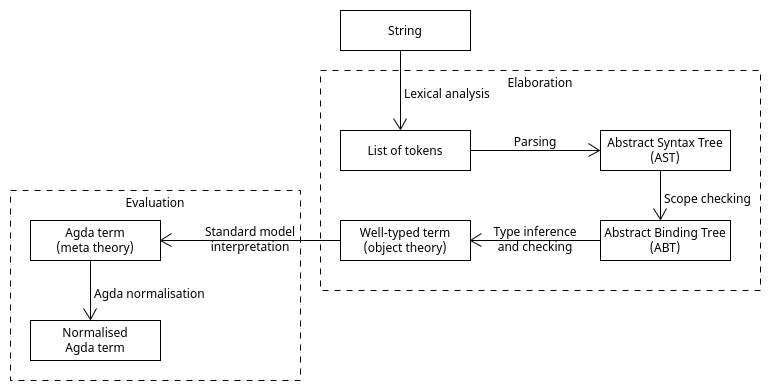
\includegraphics[width=1.0\textwidth]{../images/architecture.png}
	\caption{High-level overview of the elaboration and evaluation steps}
	\label{fig:architecture}
\end{figure}

From our seven representations: string and list of tokens are trivial; AST and ABT are simple inductive data types (albeit the latter is indexed by \verb$ℕ$); and Agda terms, whether in normal form or not, are in the metatheoretic domain, which we do not have to deal with. The well-typed term level, i.e., our object theory, is the only one that bears a more complex definition.

From the six transitions between our levels of abstractions: lexical analysis and parsing are solved in a high-level approach using the agdarsec library; scope checking, type inference and standard model interpretation bear more in-depth explanations; and Agda normalisation is again, not part of our domain.

We give prefixes to our constructors on all levels for clarity, e.g., \verb$t-true$ for the token, \verb$s-true$ for the AST (syntactic) term, \verb$p-true$ for its parser, and \verb$abt-true$ for the ABT term. Well-typed terms have no prefixes, e.g., \verb$true$. We also often use the "o" suffix for distinguishing between Agda terms and our own, e.g. in \verb$zeroo$ and \verb$suco$.

\begin{figure}[h!]
	\centering
	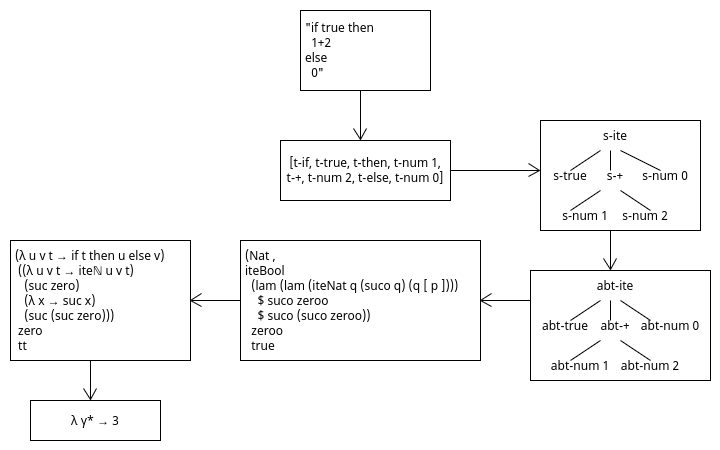
\includegraphics[width=1.0\textwidth]{../images/example-1.png}
	\caption{A simple elaboration example}
	\label{fig:example-1}
\end{figure}

\section{Lexical analysis} \label{sec:lexer}

First, it is worth mentioning that we initially implemented our own lexer, which was functionally the same as the final implementation relying on agdarsec. It was a simple algorithm: read the input by characters; accumulate them to a word until a whitespace or separator is read; if it is a valid token, put it into a list, otherwise return an error; repeat the steps until end of input.

Since agdarsec already ships with a high-level interface for lexical analysis, we chose to abstract this step similarly to parsing.

\begin{listing}[H]
\begin{minted}{agda}
data Tok : Set where
  t-true   : Tok
  t-false  : Tok
  t-if     : Tok
  t-then   : Tok
  t-else   : Tok
  t-isZero : Tok
  t-+      : Tok
  t-num    : ℕ → Tok
  t-λ      : Tok
  t-var    : String → Tok
\end{minted}
\caption{Portion from our vocabulary of tokens}
\label{code:lex-tok}
\end{listing}

We have 50 tokens in total. This includes symbols like \verb$t-dot$, \verb$t-lpar$ and \verb$t-rpar$, standing for the '.' in a \verb$λ$ binding and for the '(' and ')' parentheses, respectively. On Code \ref{code:lex-tok}, and also in other code examples to follow in our thesis, we do not list all cases, only a few that can serve as examples and the more notable ones. We insert "..." comments where code is omitted from the middle of a snippet.

Tokens that need information attached are indexed. In particular, \verb$t-num$ and \verb$t-var$ store the natural numbers and variable names read from the source code, respectively.

We supply the \verb$Token = Position × Tok$ type to the lexical analyser, so it also outputs the character positions for all tokens.

The agdarsec library requires decidable equality over our token type, which we formalise in the following way: we list all 50 cases of propositional equality and postulate that the other combinations are unequal, instead of listing all the thousand and more cases. For \verb$t-num$ and \verb$t-var$ we simply rely on the decidable equality of the \verb$Nat$ and \verb$String$ types, as well as \verb$cong$, i.e., congruence of equality in Agda.

\begin{listing}[H]
\begin{minted}{agda}
eq-tok : Decidable {A = Tok} _≡_
eq-tok t-true  t-true  = yes refl
eq-tok t-false t-false = yes refl
eq-tok t-if    t-if    = yes refl
-- ...
eq-tok (t-num n) (t-num m) with n ≟ℕ m
... | yes eq = yes (cong t-num eq)
... | no ¬eq = no λ hyp → ¬eq (cong (λ { (t-num n) → n ; _ → 0}) hyp)
eq-tok t-λ t-λ = yes refl
eq-tok (t-var name) (t-var name') with name ≟str name'
... | yes eq = yes (cong t-var eq)
... | no ¬eq = no λ hyp → ¬eq (cong (λ { (t-var s) → s ; _ → ""}) hyp)
-- ...
eq-tok _ _ = no no-more-eq where
  private postulate no-more-eq : ∀ {A} → A
\end{minted}
\caption{Decidability of token equivalence}
\label{code:lex-tok-eq}
\end{listing}

\begin{listing}[H]
\begin{minted}{agda}
keywords : List⁺ (String × Tok)
keywords = ("true", t-true) ∷ ("false", t-false) ∷ ("if", t-if) ∷ {- ... -} ∷ []
\end{minted}
\caption{Mapping strings to our token type}
\label{code:lex-keywords}
\end{listing}

\begin{listing}[H]
\begin{minted}{agda}
breaking : Char → ∃ λ b → if b then Maybe Tok else Lift _ ⊤
breaking c = case c of λ where
  '+' → true , just t-+
  'λ' → true , just t-λ
  '.' → true , just t-dot
  '→' → true , just t-→
-- ...
  c   → if isSpace c then true , nothing else false , _
\end{minted}
\caption{Special tokens that also work as separators}
\label{code:lex-breaking}
\end{listing}

As expected, all whitespace characters act as valid separators. Additionally, our tokens which are symbols, i.e., the ones that are not alphanumeric, are also accepted as separators. For example, \verb$"λx.x+10"$ is lexically valid. On Code \ref{code:lex-breaking} we can see that \verb$breaking$ takes a character and returns a pair. The first field indicates if it is a separator and the second optionally contains a \verb$Tok$ depending on whether it is also a token.

\begin{listing}[H]
\begin{minted}{agda}
default : String → Tok
default s = case (listch⇒ℕ (toList s)) of λ where
  (just n) → t-num n
  nothing  → t-var s
\end{minted}
\caption{Fallback function for words that are not keywords or separators}
\label{code:lex-default}
\end{listing}

If the lexer encounters a word that is not a valid keyword or a separator, then it calls the \verb$default$ function on it. Our implementation tests whether the word is a valid natural number. If it is, then it constructs a \verb$t-num$, otherwise we treat the word as a variable name using \verb$t-var$. \verb$listch⇒ℕ$ has a standard definition as seen on Code \ref{code:lex-reading-nat}.

\begin{listing}[H]
\begin{minted}{agda}
listch⇒ℕ : List Char → Maybe ℕ
listch⇒ℕ [] = nothing
listch⇒ℕ = step 0 where
  step : ℕ → List Char → Maybe ℕ
  step n [] = just n
  step n (c ∷ cs) = if isDigit c then
                      step (n + (pow 10 (length cs)) * (toℕ c - 48)) cs
                    else
                      nothing where
    pow : ℕ → ℕ → ℕ
    pow b = λ { 0 → 1 ; (suc e) → b * (pow b e)}
\end{minted}
\caption{Reading natural numbers from lists of characters}
\label{code:lex-reading-nat}
\end{listing}

Accepting arbitrary strings as variable names is uncommon. We chose this approach, because agdarsec's interface, i.e., the \verb$default$ function, does not support returning an error. It returns \verb$Tok$ and not a type like \verb$Maybe Tok$. We could of course return an "error token", but that would pollute our \verb$Tok$ type, and also, the error would surface during parsing, which would not be elegant. A potential clean solution would be to bring back our self-made tokenizer (that only accepted alphanumeric variable names) and inject that to agdarsec's parsing toolchain. There is support for this, and could be a potential improvement in the future.

The lexer itself is parametrized with the three functions discussed above using the \verb$import$ statement:

\mint{agda}|open import Text.Lexer keywords breaking default|

\section{Parsing}

Like with lexical analysis, our first approach was to implement our own parsing algorithm. This meant a recursive function that simulated a state machine. There were two problems with this approach. First, Agda's termination checker rejected recursive calls at binary and ternary operators, with no trivial way around it, i.e., without implementing some form of fixpoint combinator. Second, our implementation could only handle the Polish notation of STLC, i.e., operators had to be written in prefix order: \verb$+ 1 + 2 3$ instead of \verb$1 + 2 + 3$. Implementing infix syntax for operators like \verb$_+_$, function application with no symbol required, and support for parenthesis proved to be far from trivial. In essence, we would have had to implement a parser combinator library of our own. In order to avoid reinventing the wheel, we opted to use agdarsec for building our AST.

Setting up agdarsec's parser takes substantial importing and argument instancing work, mostly concerning monadic constructions. We chose to omit these implementation details from this thesis. Those who are interested can find the code in our repository \cite{home-repo}, or can see similar usages among the examples distributed with the library. Instead, we will focus on the high-level construction of the syntax itself by building and composing combinators with the library.

First, we present our syntax on Code \ref{code:parse-ast}. We have nullary nodes, like the Bool constructors \verb$s-true$, \verb$s-false$ or \verb$s-nil$, which creates the empty list. Unary nodes include the product elimination rules \verb$s-fst$ and \verb$s-snd$, and the sum introduction rules \verb$s-inl$ and \verb$s-inr$. STLC has several binary operators, for example, addition of naturals \verb$_s-+_$, function elimination \verb$_s-$\verb=$=\verb$_$, type former for products \verb$_s-,_$ or the cons operator of lists \verb$_s-∷_$. Ternary nodes include iterators like \verb$s-ite$ (this is the Bool destructor "if then else"), \verb$s-iteℕ$, \verb$s-iteList$ and \verb$s-iteTree$.

Code \ref{code:parse-stype} depicts the syntax we use for our type annotations, which we will need to clarify types of terms like the empty list \verb$"nil"$ or identity function \verb$"λx.x"$. Their code might look like \verb$"nil : [ℕ]"$ and \verb$"(λx.x) : ℕ → ℕ"$, respectively.

\begin{listing}[H]
\begin{minted}{agda}
data AST : Set where
  s-true       : AST
  s-false      : AST
  s-ite        : AST → AST → AST → AST
  s-isZero     : AST → AST
  _s-+_        : AST → AST → AST
  s-num        : ℕ → AST
  s-λ          : List String → AST → AST
  s-var        : String → AST
  _s-$_        : AST → AST → AST

  s-triv       : AST
  _s-,_        : AST → AST → AST
  s-fst        : AST → AST
  s-snd        : AST → AST

  s-inl        : AST → AST
  s-inr        : AST → AST
  s-case       : AST → AST → AST

  s-nil        : AST
  _s-∷_        : AST → AST → AST

  s-leaf       : AST → AST
  _s-node_     : AST → AST → AST

  s-iteℕ       : AST → AST → AST → AST
  s-iteList    : AST → AST → AST → AST
  s-iteTree    : AST → AST → AST → AST

  s-head       : AST → AST
  s-tail       : AST → AST
  s-genStream  : AST → AST → AST → AST

  s-put        : AST → AST → AST
  s-set        : AST → AST
  s-get        : AST → AST
  s-genMachine : AST → AST → AST → AST → AST

  s-ann        : AST → SType → AST
\end{minted}
\caption{Syntax of STLC}
\label{code:parse-ast}
\end{listing}

\begin{listing}[H]
\begin{minted}{agda}
data SType : Set where
  s-Nat     : SType
  s-Bool    : SType
  _s-→_     : SType → SType → SType
  s-⊤       : SType
  s-⊥       : SType
  _s-×_     : SType → SType → SType
  _s-⊎_     : SType → SType → SType
  s-List    : SType → SType
  s-Tree    : SType → SType
  s-Stream  : SType → SType
  s-Machine : SType
\end{minted}
\caption{Syntax for type annotations}
\label{code:parse-stype}
\end{listing}

At this level \verb$s-λ$ does not mean Church's usual lambda, but an abstract node that stores a list of variable names it binds, since we support the compact notation \verb$"λ x y z. x+y+z"$. We will unroll this to properly nested lambdas when introducing De Bruijn indices \cite{de1972lambda} on our ABT level. Analogue to this, \verb$s-var$ stores the parsed variable name in its index, which will be turned to a De Bruijn index later.

\begin{listing}[H]
\begin{minted}{agda}
p-tok : Tok → ∀[ Parser P [ Token ] ]
p-tok t = maybeTok $ λ where
  tok@(_ , t') → case eq-tok t t' of λ where
    (yes eq) → just tok
    (no ¬eq) → nothing

p-parens : ∀ {A} → ∀[ □ Parser P A ⇒ Parser P A ]
p-parens rec = p-tok t-lpar &> rec <& box (p-tok t-rpar)

p-name : ∀[ Parser P [ String ] ]
p-name = maybeTok λ where (_ , t-var s) → just s; _ → nothing
\end{minted}
\caption{Parsing exact tokens, parenthesised terms and variable names}
\label{code:parse-basic-parsers}
\end{listing}

\verb$p-tok$ parses an exact token by using \verb$eq-tok$ introduced in the previous chapter. \verb$p-parens$ parses an opening parenthesis, followed by a recursive parsing of an arbitrary term, and then by a closing parenthesis. We always call the parameter passed for recursive parsing \verb$rec$, which has type \verb$□ Parser P A$. Here, \verb$□$ means the type is "boxed" or "guarded" as in \textit{guarded recursion} \cite{veltri2019guarded}; \verb$P$ stands for the parameters of the parsing module; and \verb$A$ is an arbitrary type, so \verb$p-parens$ is polymorphic and can be used to parse any type between parentheses. \verb$p-name$ can parse arbitrary strings, which we use in \verb$p-var$ and \verb$p-λ$.

\begin{listing}[H]
\begin{minted}{agda}
p-type : ∀[ Parser P [ SType ] ]
p-type = fix _ $ λ rec →
  let p-nat     = s-Nat     <$ p-tok t-ℕ
      p-bool    = s-Bool    <$ p-tok t-𝕃
      p-unit    = s-⊤       <$ p-tok t-⊤
      p-empty   = s-⊥       <$ p-tok t-⊥
      p-machine = s-Machine <$ p-tok t-Machine
      p-list'   = s-List    <$> (p-tok t-[ &> rec <& box (p-tok t-]))

      p-atom = p-nat <|> p-bool <|> p-unit <|> p-empty <|> p-machine <|>
               p-list' <|> p-parens rec
      p-×    = chainr1 p-atom (box (_s-×_ <$ p-tok t-×))
      p-+    = chainr1 p-×    (box (_s-⊎_ <$ p-tok t-⊎))
      p-→    = chainr1 p-+    (box (_s-→_ <$ p-tok t-→))

      p-list   = s-List   <$> (p-tok t-List   &> box p-atom)
      p-tree   = s-Tree   <$> (p-tok t-Tree   &> box p-atom)
      p-stream = s-Stream <$> (p-tok t-Stream &> box p-atom)

  in p-→ <|> p-list <|> p-tree <|> p-stream
\end{minted}
\caption{Parsing type annotations}
\label{code:parse-p-type}
\end{listing}

We use agdarsec's fixpoint combinator \verb$fix$ for recursively parsing the syntax of type annotations as seen on Code \ref{code:parse-p-type}. The parsing of nullary and unary nodes are trivial, though note the required use of the \verb$box$ operator for the type correctness of the total parsing. For binary nodes \verb$p-→$, \verb$p-+$ and \verb$p-×$, we use the library's \verb$chainr1$ combinator, which parses right associative chains of operators. The order of embedding among them determines the precedence between these operators. Also, these chains can consist of single elements, and as a result, \verb$"ℕ"$ is parsed as a single-element \verb$→$ chain, of a single-element \verb$+$ chain of a single-element \verb$×$ chain of an atom, which gets accepted by \verb$p-nat$.

We guarantee guardedness by wrapping the recursive call in parentheses, i.e., the \verb$p-parens rec$ case in \verb$p-atom$. This introduces requirement for some parentheses in certain situations. However, this lifts some ambiguity, for example, in \verb$"List ℕ → 𝕃"$ between the choices of \verb$"List (ℕ → 𝕃)"$ and \verb$"(List ℕ) → 𝕃"$.

Our list types support two separate syntaxes: the classical \verb$"List ℕ"$ and the Haskell-like \verb$"[ℕ]"$.

For \verb$AST$, parsers of non-recursive nodes like \verb$p-true$, \verb$p-false$ or \verb$p-num$ have type \verb$∀[ Parser P [ AST ] ]$, while parsers of recursive nodes are \verb$∀[ □ Parser P [ AST ] ⇒ Parser P [ AST ] ]$, where the guarded parameter is the recursive parser we name \verb$rec$. Without listing them all, we include a few more examples on Code \ref{code:parse-some-parsers}.

\begin{listing}[H]
\begin{minted}{agda}
p-λ rec = (λ l⁺ → s-λ (toList l⁺)) <$>
          (p-tok t-λ &> box (list⁺ p-name) <& box (p-tok t-dot)) <*> rec

p-$ rec = _s-$_ <$> p-subexp rec <*> rec

p-+ rec = chainl1 (p-subexp rec) (box (_s-+_ <$ p-tok t-+))
p-, rec = chainr1 (p-+ rec)      (box (_s-,_ <$ p-tok t-,))
p-∷ rec = chainr1 (p-, rec)      (box (_s-∷_ <$ p-tok t-∷))

p-list rec = (add-nil <$> (p-tok t-[ &> box (chainr1 (p-subexp rec)
             (box (_s-∷_ <$ p-tok t-,))) <& box (p-tok t-])))
             <|>
             (s-nil <$ p-tok t-[ <& box (p-tok t-])) where
  add-nil : AST → AST
  add-nil (l s-∷ r) = l s-∷ (add-nil r)
  add-nil = _s-∷ s-nil

p-ann rec = s-ann <$> p-subexp rec <*> box (p-tok t-: &> box p-type)
\end{minted}
\caption{Parsers of some nodes in our AST}
\label{code:parse-some-parsers}
\end{listing}

There is no combinator in agdarsec that would allow us writing a parser that accepts an empty input, or an empty list to be more precise, since non-advancing parsers would violate totality. This aligns with our need for \verb$s-λ$, since we expect at least one variable name to bind in a lambda expression. For this, we use the \verb$list⁺$ combinator. Converting it back to a simple list with \verb$toList$ is just an implementation trick, a liberty we took, so we could more easily pattern match later in the scope checking step.

The case of \verb$p-∷$, \verb$p-,$ and \verb$p-+$ is similar to the binary nodes presented in our \verb$p-type$ example.

In \verb$p-list$ we handle the empty list and non-empty list cases separately. Since we cannot have a parser that accepts the empty string, we need to manually add \verb$nil$ to the end of our non-empty list case using \verb$add-nil$.

Finally, to conclude our parsing stack, we present the definitions of \verb$p-subexp$ and \verb$p-exp$ on Code \ref{code:parse-p-exp}.

\begin{listing}[H]
\begin{minted}{agda}
p-subexp rec =
  p-true       <|>
  p-false      <|>
  p-num        <|>
  p-var        <|>
  p-triv       <|>
  p-nil        <|>
  p-leaf   rec <|>
  p-parens rec

p-exp = fix _ $ λ rec →
  p-ann        rec <|>
  p-list       rec <|>
  p-node       rec <|>
  p-$          rec <|>
  p-∷          rec <|>
  p-ite        rec <|>
  p-isZero     rec <|>
  p-fst        rec <|>
  p-snd        rec <|>
  p-inl        rec <|>
  p-inr        rec <|>
  p-case       rec <|>
  p-λ          rec <|>
  p-iteℕ       rec <|>
  p-iteList    rec <|>
  p-iteTree    rec <|>
  p-head       rec <|>
  p-tail       rec <|>
  p-genStream  rec <|>
  p-put        rec <|>
  p-set        rec <|>
  p-get        rec <|>
  p-genMachine rec <|>
  p-subexp     rec
\end{minted}
\caption{p-subexp and p-exp parsers}
\label{code:parse-p-exp}
\end{listing}

\verb$p-subexp$ has all nullary nodes listed, because they don't need to be guarded by parentheses. \verb$p-leaf$ is included too, since it is guarded in itself, because of its unique prefix, e.g., leaves of \verb$Tree ℕ$ look like \verb$"<42>"$. \verb$p-exp$ is the top-level parser of STLC.

Omitting the cumbersome work of argument instancing, we show the final parsing algorithm on Code \ref{code:parse-algo}.

\begin{listing}[H]
\begin{minted}{agda}
module _ (open Parameters P)
  -- ...
  parse_by_ : ∀ {A : Set≤ l} → String → ∀[ Parser P A ] → Maybe (theSet A)
  parse s by parser =
   let input = Vec.fromList $ Tokenizer.fromText t s
       parse = runParser parser (n≤1+n _) (lift $ 𝕃.into input)
       check = λ s → if ⌊ Success.size s Nat.≟ 0 ⌋
                     then just (Success.value s) else nothing
   in case List.TraversableM.mapM MaybeCat.monad check $ runM ℝ parse of λ where
        (just (a ∷ _)) → just (lower a)
        _              → nothing
  parse-exp : String → Maybe AST
  parse-exp s = parse s by p-exp

parse : String → Maybe AST
parse = parse-exp
\end{minted}
\caption{Monadic total implementation of the parsing stack}
\label{code:parse-algo}
\end{listing}

Without going too much into detail, we can see that our function starts from a string (the source code) and a parser (\verb$p-exp$ in our case). It runs the injected tokenizer, for which we use the one provided by agdarsec, parametrized with our three functions discussed in the previous chapter. It is also clear that the parsing can fail, which is indicated by returning \verb$nothing$. The need for the \verb$n≤1+n$ proof suggests that the internal code of agdarsec uses the fact that parsing always consumes some non-zero amount of characters from the input, thus reducing the sized type used.

\begin{listing}[H]
\begin{minted}{agda}
_ : parse "10 + 20 + 30"   ≡ just (s-num 10 s-+ s-num 20 s-+ s-num 30)
_ = refl
_ : parse "(10 + 20) + 30" ≡ just ((s-num 10 s-+ s-num 20) s-+ s-num 30)
_ = refl
_ : parse "10 + (20 + 30)" ≡ just (s-num 10 s-+ (s-num 20 s-+ s-num 30))
_ = refl
_ : parse "λ f x. if f x then x else 0" ≡
          just (s-λ ("f" ∷ "x" ∷ []) (s-ite (s-var "f" s-$ s-var "x")
                                            (s-var "x") (s-num 0)))
_ = refl
\end{minted}
\caption{Parsing examples}
\label{code:parse-examples}
\end{listing}

\section{Scope checking}

\begin{listing}[H]
\begin{minted}{agda}
data ABT (n : ℕ) : Set where
  abt-true       : ABT n
  abt-false      : ABT n
  abt-ite        : ABT n → ABT n → ABT n → ABT n
  abt-isZero     : ABT n → ABT n
  _abt-+_        : ABT n → ABT n → ABT n
  abt-num        : ℕ → ABT n
  abt-λ          : ABT (suc n) → ABT n
  _abt-$_        : ABT n → ABT n → ABT n
  abt-var        : Fin n → ABT n

  abt-triv       : ABT n
  _abt-,_        : ABT n → ABT n → ABT n
  abt-fst        : ABT n → ABT n
  abt-snd        : ABT n → ABT n

  abt-inl        : ABT n → ABT n
  abt-inr        : ABT n → ABT n
  abt-case       : ABT n → ABT n → ABT n

  abt-nil        : ABT n
  _abt-∷_        : ABT n → ABT n → ABT n

  abt-leaf       : ABT n → ABT n
  _abt-node_     : ABT n → ABT n → ABT n

  abt-iteℕ       : ABT n → ABT n → ABT n → ABT n
  abt-iteList    : ABT n → ABT n → ABT n → ABT n
  abt-iteTree    : ABT n → ABT n → ABT n → ABT n

  abt-head       : ABT n → ABT n
  abt-tail       : ABT n → ABT n
  abt-genStream  : ABT n → ABT n → ABT n → ABT n

  abt-put        : ABT n → ABT n → ABT n
  abt-set        : ABT n → ABT n
  abt-get        : ABT n → ABT n
  abt-genMachine : ABT n → ABT n → ABT n → ABT n → ABT n

  abt-ann        : ABT n → SType → ABT n
\end{minted}
\caption{Syntax for abstract binding trees of STLC}
\label{code:abt-def}
\end{listing}

The most apparent difference between our AST and ABT definitions is that the latter is indexed by \verb$ℕ$. This index indicates the number of free variables in the expression, i.e., the size of context the corresponding typed term needs.

Another notable difference is in \verb$abt-λ$. It no longer stores the list of variable names obtained from the source code. Instead, we unroll these shorthand lambdas to separate constructors, which we will treat as binders that use De Bruijn indices \cite{de1972lambda}. For example, \verb$s-λ ("x" ∷ "y" ∷ []) (s-var "x" s-+ s-var "y")$ is turned into \verb$abt-λ (abt-λ (abt-var 1 abt-+ abt-var 0))$. Note that the first variable, \verb$x$, got the index one, and \verb$y$ got index zero. This is because De Bruijn indices indicate the \textit{distance} from the represented variable's binder in the tree.

Naturally, our \verb$abt-var$ node is also indexed by natural numbers instead of strings. To be more rigorous, we chose to use \verb$Fin n$ (set of n elements, i.e., subset of naturals from 0 to n-1) in our definition \verb$abt-var : Fin n → ABT n$, as can be seen on Code \ref{code:abt-def}. This ensures that we cannot create an ABT which has a variable reference that is out of bounds, i.e., one that uses an index not present in its context.

Our scope checking formalisation rely on a few lemmas depicted on Codes \ref{code:abt-lift-abt} and \ref{code:abt-arit-lemmas}. Here we omit the proofs for the arithmetic ones, but they can be found in our codebase.

\begin{listing}[H]
\begin{minted}{agda}
lift-abt : {m n : ℕ} → (m ≤ n) → ABT m → ABT n
lift-abt m≤n (u abt-+ v) = (lift-abt m≤n u) abt-+ (lift-abt m≤n v)
lift-abt m≤n (abt-num n) = abt-num n
lift-abt m≤n (abt-λ t)   = abt-λ (lift-abt m≤n t)
lift-abt m≤n (u abt-$ v) = (lift-abt m≤n u) abt-$ (lift-abt m≤n v)
lift-abt {m} {n} m≤n (abt-var f) = abt-var (inject≤ {m} {n} f m≤n) where
  inject≤ : {m n : ℕ} → Fin m → m ≤ n → Fin n
  inject≤ {_} {suc n} zero    _     = Fin.zero
  inject≤ {_} {suc n} (suc i) (m≤n) = suc (inject≤ i m≤n)
-- ...
\end{minted}
\caption{Lemma: an ABT can always be embedded into a bigger context}
\label{code:abt-lift-abt}
\end{listing}

\begin{listing}[H]
\begin{minted}{agda}
≤-max2 : (n m : ℕ) → (n ≤ max n m) ×
                     (m ≤ max n m)

≤-max3 : (n m k : ℕ) → (n ≤ max (max n m) k) ×
                       (m ≤ max (max n m) k) ×
                       (k ≤ max (max n m) k)

≤-max4 : (n m k l : ℕ) → (n ≤ max (max (max n m) k) l) ×
                         (m ≤ max (max (max n m) k) l) ×
                         (k ≤ max (max (max n m) k) l) ×
                         (l ≤ max (max (max n m) k) l)
\end{minted}
\caption{Arithmetic lemmas needed for scope checking}
\label{code:abt-arit-lemmas}
\end{listing}

\begin{listing}[H]
\begin{minted}{agda}
scopeinfer : AST → Maybe (Σ ℕ λ n → ABT n)
scopeinfer = sinfer [] where

  sinfer : List String → AST → Maybe (Σ ℕ λ n → ABT n)

  sinfer ss s-true  = just (0 , abt-true)
  sinfer ss s-false = just (0 , abt-false)

  sinfer ss (s-ite t u v) with sinfer ss t | sinfer ss u | sinfer ss v
  ... | just (i , t') | just (j , u') | just (k , v') =
  just (max (max i j) k , abt-ite (lift-abt (π₁     (≤-max3 i j k))  t')
                                  (lift-abt (π₁ (π₂ (≤-max3 i j k))) u')
                                  (lift-abt (π₂ (π₂ (≤-max3 i j k))) v'))
  ... | _ | _ | _ = nothing
-- ...
  sinfer ss (s-λ       [] t) = sinfer ss t
  sinfer ss (s-λ (v ∷ vs) t) with sinfer (v ∷ ss) (s-λ vs t)
  ... | just (0     , t') = just (0 , abt-λ (lift-abt tt t'))
  ... | just (suc n , t') = just (n , abt-λ t')
  ... | nothing = nothing

  sinfer ss (u s-$ v) with sinfer ss u | sinfer ss v
  ... | just (i , u') | just (j , v') =
  just (max i j , _abt-$_ (lift-abt (π₁ (≤-max2 i j)) u')
                          (lift-abt (π₂ (≤-max2 i j)) v'))
  ... | _ | _ = nothing

  sinfer ss (s-var name) = case (lookup ss name) of λ where
    nothing  → nothing -- not in scope
    (just i) → just (suc i , abt-var (fromℕ i)) where
      fromℕ : (n : ℕ) → Fin (suc n)
      fromℕ = λ { 0 → Fin.zero ; (suc n) → suc (fromℕ n) }
\end{minted}
\caption{Scope inference algorithm}
\label{code:abt-scopeinfer}
\end{listing}

\verb$scopeinfer$ takes an \verb$AST$, then if it is well-scoped, it returns a dependent pair: some natural \verb$n$ and an \verb$ABT n$, otherwise it returns \verb$nothing$. Basically, what happens is that we decorate our syntax tree with context size indices. We use \verb$sinfer$ as a helper function to iterate over the tree. It accumulates the bound variable names in its first argument from the \verb$s-λ$ nodes. Then, at \verb$s-var$ nodes we look up the variable from the list: if not found, we return with error; otherwise we use the resulting list index as the De Bruijn index. Note that the \verb$suc$ for the ABT index is needed here only because \verb$lookup$ indexes from zero, i.e., a De Bruijn index 0 means that we need a context of at least size one.

For nodes with arity two or more, such as \verb$_s-$\verb=$=\verb$_$ and \verb$s-ite$ on Code \ref{code:abt-scopeinfer}: we recursively infer the scope of all subterms; choose the biggest scope size among them; then lift all operands to that scope for constructing the ABT node. To achieve this, we use our lemmas \verb$≤-max2$ and \verb$≤-max3$, which state that the maximum of two or three numbers is always larger than or equal to the individual numbers.

\begin{listing}[H]
\begin{minted}{agda}
scopecheck : AST → Maybe (ABT 0)
scopecheck ast with scopeinfer ast
... | just (0 , abt) = just abt
... | _              = nothing
\end{minted}
\caption{Scope checking algorithm}
\label{code:abt-scopecheck}
\end{listing}

The module's top-level function \verb$scopecheck$ simply runs the scope inference and checks whether we get a closed term, i.e., a binding tree with index zero. This is to ensure that there are no free variables in the term, or in other words: it is well-scoped. Note that, again, we encode a strong requirement in our type: the scope checking cannot return a badly scoped tree by definition.

\begin{listing}[H]
\begin{minted}{agda}
_ : scopecheck (s-var "foo") ≡ nothing
_ = refl
_ : scopecheck (s-λ ("foo" ∷ []) (s-var "bar")) ≡ nothing
_ = refl
_ : scopecheck (s-λ ("foo" ∷ []) (s-var "foo")) ≡ just (abt-λ (abt-var Fin.zero))
_ = refl
_ : scopecheck (s-λ ("x" ∷ "y" ∷ []) (s-var "x" s-+ s-var "y")) ≡
               just (abt-λ (abt-λ (abt-var (suc Fin.zero) abt-+ abt-var Fin.zero)))
_ = refl
\end{minted}
\caption{Scope checking examples}
\label{code:abt-scopecheck-ex}
\end{listing}

\newpage

\section{Bidirectional type checking} \label{sec:typecheck}

In this chapter, we first give a brief introduction to our well-typed syntax for easier understanding. However, we will discuss our object theory in more detail in the next chapter.

\begin{listing}[H]
\begin{minted}{agda}
data Ty   : Set where
  _⇒_     : Ty → Ty → Ty
  _×o_    : Ty → Ty → Ty
  Unit    : Ty
  _+o_    : Ty → Ty → Ty
  Empty   : Ty
  Bool    : Ty
  Nat     : Ty
  List    : Ty → Ty
  Tree    : Ty → Ty
  Stream  : Ty → Ty
  Machine : Ty

data Con : Set where
  ◇      : Con
  _▹_    : Con → Ty → Con

Tm : Con → Ty → Set
-- ...
\end{minted}
\caption{Types, contexts and terms in the well-typed syntax}
\label{code:typecheck-ty}
\end{listing}

Not surprisingly, \verb$Ty$ has the exact same definition as our syntactic types, \verb$SType$, as visible when comparing Code \ref{code:parse-stype} with \ref{code:typecheck-ty}. Contexts, \verb$Con$, are simply a list of types, where \verb$◇$ corresponds to nil, and \verb$_▹_$ is similar to the cons constructor, takes a prefix list and a type to form a new context. So \verb$◇$ represents the empty context, and \verb$◇ ▹ Nat ▹ Bool$ stands for the context that has a \verb$Bool$ and a \verb$Nat$ variable in De Bruijn indices zero and one, respectively. The indices are inverted, because when we append a new variable with a \verb$λ$ introduction, it becomes De Bruijn index zero.

Terms, \verb$Tm$, are indexed by their contexts and their types. Later we will see that we cannot construct arbitrary terms from arbitrary contexts. For example, the term \verb$q$, which stands for the "last bound variable", cannot be constructed in the empty context.

Codes \ref{code:typecheck-ty-eq}, \ref{code:typecheck-infer-ty} and \ref{code:typecheck-helpers} show portions from code used for type checking: decidable equality over \verb$Ty$; mapping from the syntactic \verb$SType$ to \verb$Ty$; and a few additional helper functions, respectively.

\begin{listing}[H]
\begin{minted}{agda}
_≟_ : (A B : Ty) → Dec (A ≡ B)
Nat  ≟ Nat      = yes refl
Nat  ≟ Bool     = no λ ()
Nat  ≟ Unit     = no λ ()
Nat  ≟ Empty    = no λ ()
Nat  ≟ (_ ⇒  _) = no λ ()
Nat  ≟ (_ ×o _) = no λ ()
Nat  ≟ (_ +o _) = no λ ()
-- ...
(A₁ ×o A₂) ≟ (B₁ ×o B₂) with A₁ ≟ B₁ | A₂ ≟ B₂
... | yes e₁ | yes e₂ = yes (cong₂ _×o_ e₁ e₂)
... | yes e₁ | no ¬e₂ = no λ hyp → ¬e₂ (cong ×snd hyp) where
  ×snd : Ty → Ty
  ×snd = λ { (A ×o B) → B ; X → X }
... | no ¬e₁ | yes e₂ = no λ hyp → ¬e₁ (cong ×fst hyp) where
  ×fst : Ty → Ty
  ×fst = λ { (A ×o B) → A ; X → X }
... | no ¬e₁ | no ¬e₂ = no λ hyp → ¬e₁ (cong ×fst hyp) where
  ×fst : Ty → Ty
  ×fst = λ { (A ×o B) → A ; X → X }
-- ...
\end{minted}
\caption{Decidable equality of types}
\label{code:typecheck-ty-eq}
\end{listing}

\begin{listing}[H]
\begin{minted}{agda}
infer-ty : SType → Maybe Ty
infer-ty s-Nat  = just Nat
infer-ty s-Bool = just Bool
infer-ty s-⊤    = just Unit
infer-ty s-⊥    = just Empty
infer-ty (A s-→ B) with infer-ty A | infer-ty B
... | just A' | just B' = just (A' ⇒ B')
... | _       | _       = nothing
\end{minted}
\caption{Mapping syntactic types SType to Ty}
\label{code:typecheck-infer-ty}
\end{listing}

\begin{listing}[H]
\begin{minted}{agda}
length : Con → ℕ
length = λ { ◇ → 0 ; (Γ ▹ _) → suc (length Γ) }

lookup : (Γ : Con) → Fin (length Γ) → (Σ Ty λ A → Tm Γ A)
lookup (Γ ▹ A) zero    = A , q
lookup (Γ ▹ A) (suc n) = proj₁ rest , proj₂ rest [ p ] where
  rest : Σ Ty λ A → Tm Γ A
  rest = lookup Γ n

fconv : {Γ : Con}{A B : Ty} → Tm Γ (A ⇒ B) → Tm (Γ ▹ A) B
fconv f = f [ p ] $ q
\end{minted}
\caption{Helper functions for type checking}
\label{code:typecheck-helpers}
\end{listing}

\verb$lookup$ is a safe function, due to the index argument's type \verb$Fin (length Γ)$, that searches the nth type from a \verb$Con$. It also constructs the term that extracts said nth variable from the context. For this, it builds a chain of \verb$[ p ]$ substitutions with length equal to the queried index. Informally, all \verb$[ p ]$ substitutions "peel off" the last bound variable from the list. Finally, the function puts a \verb$q$ to the term, that extracts the last variable from the truncated list. For example, if we run \verb$lookup Γ 3$, then we get a pair like: \verb$A , q [ p ] [ p ] [ p ]$, where \verb$A$ is the type of the variable at De Bruijn index three in \verb$Γ$. We have a shorthand notation for the previous term: \verb$q [ p ⊚ p ⊚ p ]$.

\verb$fconv$ is interesting when we consider our introduction rule for abstraction:
\mint{agda}|lam : ∀{Γ A B} → Tm (Γ ▹ A) B → Tm Γ (A ⇒ B)|
\noindent{It means that when we can explain a term of type \verb$B$ using a context that is some \verb$Γ$ plus a variable \verb$A$, we can also always explain a function in context \verb$Γ$ that goes from \verb$A$ to \verb$B$. \verb$fconv$ proves the opposite direction by weakening the function's context in \verb$f [ p ]$ and then applying the first variable from this context to it with \verb$$\verb=$=\verb$ q$. We explain \verb$q$, \verb$p$, \verb$_[_]$ and \verb$_$\verb=$=\verb$_$, alongside the whole substitution calculus, in Chapter \ref{sec:algebraic-def} in more detail.

\noindent{\textit{Corollary:} \verb$Tm (Γ ▹ A) B$ and \verb$Tm Γ (A ⇒ B)$ are isomorphic in our model.}}

Note the difference between \verb$→$ and \verb$⇒$ in the above definition. The former denotes function types in our metatheoretic language, while the latter means functions in our object theory.

Bidirectional type checking consists of the usual \cite{dunfield2021bidirectional} two functions: \verb$infer$ and \verb$check$. Both take an ABT term as input. The former, if well-typed, returns its inferred type and the corresponding well-typed term. The latter takes the expected type as argument and checks whether the input term has said type; if yes, it returns the well-typed term.

\begin{listing}[H]
\begin{minted}{agda}
infer : (Γ : Con) → ABT (length Γ) → Maybe (Σ Ty λ A → Tm Γ A)
check : (Γ : Con) → (A : Ty) → ABT (length Γ) → Maybe (Tm Γ A)
\end{minted}
\caption{Types of functions infer and check}
\label{code:typecheck-signatures}
\end{listing}

From Code \ref{code:typecheck-infer-triv} to \ref{code:typecheck-check-ann}, we present a non-exhaustive subset of our inference and checking rules.

\begin{listing}[H]
\begin{minted}{agda}
infer Γ abt-true  = just (Bool , true)
infer Γ abt-false = just (Bool , false)

infer Γ (abt-isZero t) with infer Γ t
... | just (Nat , t') = just (Bool , iteNat true false t')
... | _               = nothing
\end{minted}
\caption{Type inference: some trivial cases}
\label{code:typecheck-infer-triv}
\end{listing}

It is a recurring pattern that type inference of terms usually requires type inference of their subterm(s), like with \verb$isZero$, where the subterm must be a \verb$Nat$.

\begin{listing}[H]
\begin{minted}{agda}
infer Γ (abt-ite t u v) with infer Γ t | infer Γ u | infer Γ v
... | just (Bool , t') | just (A , u') | just (B , v') with B ≟ A
... | yes e = just (A , iteBool u' (transp (λ X → Tm Γ X) e v') t')
... | _     = nothing
infer Γ (abt-ite t u v) | _ | _ | _ = nothing

infer Γ (u abt-+ v) with infer Γ u | infer Γ v
... | just (Nat , u') | just (Nat , v') = just (Nat , iteNat v' (suco q) u')
... | _               | _               = nothing
\end{minted}
\caption{Type inference: if-then-else and addition}
\label{code:typecheck-infer-ite}
\end{listing}

For \verb$"if t then u else v"$ constructions, we first check whether \verb$t$ is of type \verb$Bool$ and that \verb$u$ and \verb$v$ have the same type by using pattern matching. If all criteria hold, we use \verb$Bool$'s iterator \verb$iteBool$ for building the well-typed term. It normalises to its first argument if the third does to \verb$true$, or to the second otherwise. The use of \verb$transp$ in this proof and in ones to follow is simply needed for technical reasons.
\mint{agda}|transp : ∀{ℓ}{A : Set ℓ}{ℓ'}(P : A → Set ℓ'){a a' : A} → a ≡ a' → P a → P a'|
With this, we can transport propositions over \textit{propositional equality} of \verb$Ty$, because Agda does this implicitly only with its own \textit{definitional equality}. More precisely, if we have a proof for \verb$a ≡ a'$ and that \verb$P a$ holds, \verb$transp$ gives us a proof of \verb$P a'$. So here we rely on the correctness of the trivial \verb$≟$ proposition of \verb$Ty$ equality from before.

The addition operator is handled similarly, now using the iterator of naturals, \verb$iteNat$. Its first argument is the term that \verb$zeroo$ will be replaced with; the second is one that given a partial result of the iteration (in the context), produces the next result for each \verb$suco$; and the third is the \verb$Nat$ that we wish to iterate on.
\mint{agda}|iteNat : ∀{Γ A} → Tm Γ A → Tm (Γ ▹ A) A → Tm Γ Nat → Tm Γ A|
In case of our addition, we replace the \verb$zeroo$ in the first number with the second number itself, then for each \verb$suco$ in the first number we insert a \verb$suco$ into the result.

\begin{listing}[H]
\begin{minted}{agda}
infer Γ (abt-λ t) = nothing

infer Γ (u abt-$ v)     with infer Γ u
... | just (A ⇒ B , u') with check Γ A v
... | just v' = just (B , u' $ v')
... | nothing = nothing
infer Γ (u abt-$ v) | _ = nothing

infer Γ (abt-var n) = just (lookup Γ n)
\end{minted}
\caption{Type inference: abstraction, application and variable lookup}
\label{code:typecheck-infer-lam}
\end{listing}

We reject inference of abstractions by returning \verb$nothing$, because we cannot determine types of bound variables in general. For example, the type of \verb$"λx.x"$ can be \verb$"ℕ → ℕ"$, \verb$"𝕃 → 𝕃"$, \verb$"[ℕ] → [ℕ]"$ or an infinite amount of other types. It is not only the identity function that is problematic. Any abstraction that does not use all its bound variable(s) has a similar issue, like \verb$"λx.10"$, which can be \verb$"ℕ → ℕ"$, \verb$"𝕃 → ℕ"$, \verb$"⊤ → ℕ"$, etc. As a result, lambdas need to be type annotated in our language, or they must be present in a context where we expect a specific type of function through the usage of our \verb$check$ function.

When inferring an application, we first test whether the left-hand side is some function \verb$A ⇒ B$, then we check if the right-hand side is of type \verb$A$. If these hold, we can construct the term for application using \verb$$\verb=$=\verb$$.

\begin{listing}[H]
\begin{minted}{agda}
infer Γ (u abt-∷ v) with infer Γ u
... | just (A , u') with check Γ (Ty.List A) v
... | just v' = just (Ty.List A , cons u' v')
... | nothing = nothing
infer Γ (u abt-∷ v) | _ = nothing

check Γ (List A) abt-nil = just nil

check Γ A t with infer Γ t
... | nothing = nothing
... | just (B , t') with B ≟ A
... | yes e = just (transp (λ X → Tm Γ X) e t')
... | _     = nothing
\end{minted}
\caption{Type inference and checking: lists}
\label{code:typecheck-infercheck-lists}
\end{listing}

We present the mutually recursive nature of \verb$infer$ and \verb$check$ on our list type.

For determining the type of \verb$u ∷ v$, we first infer the type of the head, \verb$u$, which will be some type \verb$A$. Then we check if the rest of the list, \verb$v$, is of type \verb$List A$. If \verb$v$ is still a non-empty list, then our third case from Code \ref{code:typecheck-infercheck-lists} will run, which simply calls inference on the remainder list. \verb$infer$ and \verb$check$ will call each other, until we reach our base case: the empty list. It is clear from the code attached above, that no matter what type \verb$A$ is in \verb$List A$, we can always construct the term \verb$nil$ for any such type. This is guaranteed by Agda's polymorphic nature as our meta language:
\mint{agda}|nil : ∀{Γ A} → Tm Γ (List A)|

\verb$List$ is not the only type former, for which we need explicit \verb$check$ cases, Code \ref{code:typecheck-check-etc} shows a few more.

\begin{listing}[H]
\begin{minted}{agda}
check Γ (A ⇒ B) (abt-λ t) with check (Γ ▹ A) B t
... | just t' = just (lam t')
... | nothing = nothing

check Γ (A +o _) (abt-inl t) with infer Γ t
... | just (B , t') with B ≟ A
... | yes e = just (inl (transp (λ X → Tm Γ X) e t'))
... | _     = nothing
check Γ (A +o _) (abt-inl t) | nothing = nothing

check Γ (_ +o A) (abt-inr t) with infer Γ t
... | just (B , t') with B ≟ A
... | yes e = just (inr (transp (λ X → Tm Γ X) e t'))
... | _     = nothing
check Γ (_ +o A) (abt-inr t) | nothing = nothing
\end{minted}
\caption{Type checking: functions and sums}
\label{code:typecheck-check-etc}
\end{listing}

Some \verb$abt-λ t$ term will be a valid term of \verb$A ⇒ B$ in context \verb$Γ$, if and only if \verb$t$ is a valid term of type \verb$B$ in context \verb$(Γ ▹ A)$. The extended context here contains the variable bound by the lambda.

Sum types are introduced by the left and right injection rules \verb$inl$ and \verb$inr$. With the \verb$(A +o _)$ and \verb$(_ +o A)$ patterns in the above snippet, we indicate that the type checking does not care about the other type in the sum in these cases, respectively.

For annotated terms, we first use \verb$infer-ty$ to determine the type from the syntactic annotation. Then, we test whether the subject term has that type using \verb$check$, which simply involves an equality test of \verb$Ty$, as seen on Code \ref{code:typecheck-check-ann}.

\begin{listing}[H]
\begin{minted}{agda}
infer Γ (abt-ann t ty) with infer-ty ty
... | just A           with check Γ A t
... | just t' = just (A , t')
... | nothing = nothing
infer Γ (abt-ann t ty) | nothing = nothing

check Γ A (abt-ann t ty) with infer Γ (abt-ann t ty)
... | just (B , t') with B ≟ A
... | yes e = just (transp (λ X → Tm Γ X) e t')
... | no ¬e = nothing
check Γ A (abt-ann t ty) | nothing = nothing
\end{minted}
\caption{Type inference and checking: annotated terms}
\label{code:typecheck-check-ann}
\end{listing}

\section{Algebraic definition quotiented by equations} \label{sec:algebraic-def}

We do not include the whole formalisation of our models in this and the following chapter since that would entail depicting nearly a thousand lines of code. Instead, we highlight the most fundamental and significant parts of our code, and expect the reader to visit our codebase if they desire a deeper review.

In Chapter \ref{sec:typecheck}, we already introduced the reader to some of the concepts in our object theory, such as \verb$Ty$, \verb$Con$ and \verb$Tm$. Now we will explain the full substitution calculus and some other quotients that formalise desired \verb$β$ and \verb$η$ equivalences between terms of our language. Structures like these are sometimes called \textit{quotient inductive-inductive types}, or QIITs \cite{altenkirch2018quotient}.

Each \verb$λ$-abstraction binds a variable, introducing a new scope. We can mathematically express this using substitutions. Usual notations for rewriting \verb$(λx.M)N$ to substitution form include \verb$M[x := N]$ and \verb$M[x ↤ N]$. This means that we replace all occurrences of the variable \verb$x$ in \verb$M$ with \verb$N$. If we have a scope with multiple bound variables, e.g., \verb$(λx.(λy.(λz.M))) N₁ N₂ N₃$, we may write \verb$M[x := N₁, y := N₂, z := N₃]$. However on this level, we use De Bruijn indices, so we can omit the variable names: \verb$M[N₁, N₂, N₃]$. The notation we employ is \verb$t [u ,o v ,o w]$, since we use the letters \verb$t$, \verb$u$, \verb$v$, etc., for terms and \verb$,o$ for syntactic distinction between our object and meta languages.

\begin{listing}[H]
\begin{minted}{agda}
Sub  : Con → Con → Set
_⊚_  : ∀{Γ Δ Θ} → Sub Δ Γ → Sub Θ Δ → Sub Θ Γ
ass  : ∀{Γ Δ Θ Ξ}{γ : Sub Δ Γ}{δ : Sub Θ Δ}{θ : Sub Ξ Θ} → (γ ⊚ δ) ⊚ θ ≡ γ ⊚ (δ ⊚ θ)
id   : ∀{Γ} → Sub Γ Γ
idl  : ∀{Γ Δ}{γ : Sub Δ Γ} → id ⊚ γ ≡ γ
idr  : ∀{Γ Δ}{γ : Sub Δ Γ} → γ ⊚ id ≡ γ

ε    : ∀{Γ} → Sub Γ ◇
◇η   : ∀{Γ}{σ : Sub Γ ◇} → σ ≡ ε

Tm   : Con → Ty → Set
_[_] : ∀{Γ Δ A} → Tm Γ A → Sub Δ Γ → Tm Δ A
[∘]  : ∀{Γ Δ Θ A}{t : Tm Γ A}{γ : Sub Δ Γ}{δ : Sub Θ Δ} →  t [ γ ⊚ δ ] ≡ t [ γ ]
                                                                           [ δ ]
[id] : ∀{Γ A}{t : Tm Γ A} → t [ id ] ≡ t
_,o_ : ∀{Γ Δ A} → Sub Δ Γ → Tm Δ A → Sub Δ (Γ ▹ A)
p    : ∀{Γ A} → Sub (Γ ▹ A) Γ
q    : ∀{Γ A} → Tm (Γ ▹ A) A
▹β₁  : ∀{Γ Δ A}{γ : Sub Δ Γ}{t : Tm Δ A} → p ⊚ (γ ,o t) ≡ γ
▹β₂  : ∀{Γ Δ A}{γ : Sub Δ Γ}{t : Tm Δ A} → q [ γ ,o t ] ≡ t
▹η   : ∀{Γ Δ A}{γa : Sub Δ (Γ ▹ A)} → p ⊚ γa ,o q [ γa ] ≡ γa
\end{minted}
\caption{The substitution calculus}
\label{code:ot-subst-calc}
\end{listing}

Code \ref{code:ot-subst-calc} shows that substitution, \verb$Sub$, is between contexts, \verb$Con$s. The above explained notation appears in \verb$_[_]$. It means that if we have a term of type \verb$A$ in context \verb$Γ$ and a substitution from \verb$Δ$ to \verb$Γ$, then we can construct a term of type \verb$A$ in \verb$Δ$. This operator is often called \textit{instantiation}.

Substitutions can be composed with the \verb$_⊚_$ operator, which is associative, shown by \verb$ass$. \verb$[∘]$ says that two consecutive substitutions are equivalent to the single substitution of their composition. We call the substitution that leaves the context untouched \verb$id$. It is both a left and right identity of composition witnessed by \verb$idl$ and \verb$idr$, respectively. \verb$[id]$ states that substitution with the identity does not change any term.

\verb$ε$ means that we can substitute any \verb$Γ$ to the empty context. The uniqueness rule \verb$◇η$ states that there is exactly one such substitution.

We gave an informal introduction to \verb$p$ and \verb$q$ in the previous chapter. Their \textit{computation rules} or \textit{beta-rules} - i.e., descriptions of what happens when we apply a destructor to a constructor - formally states what we explained. \verb$p$ removes the last bound variable, returning a truncated context; and \verb$q$ extracts the last variable. Both work only on non-empty contexts as seen in the common pattern \verb$γ ,o t$.

Finally, we need one more uniqueness rule, \verb$▹η$. It describes that, given an arbitrary context, if we remove then reinsert the last variable, the result will only be equivalent to the original context.

Note that the above presented model is also often called a simply typed category with families, sCwF \cite{castellan2021categories}.

\begin{listing}[H]
\begin{minted}{agda}
lam   : ∀{Γ A B} → Tm (Γ ▹ A) B → Tm Γ (A ⇒ B)
_$_   : ∀{Γ A B} → Tm Γ (A ⇒ B) → Tm Γ A → Tm Γ B
⇒β    : ∀{Γ A B}{t : Tm (Γ ▹ A) B}{u : Tm Γ A} → lam t $ u ≡ t [ id ,o u ]
⇒η    : ∀{Γ A B}{t : Tm Γ (A ⇒ B)} → lam (t [ p ] $ q) ≡ t
lam[] : ∀{Γ A B}{t : Tm (Γ ▹ A) B}{Δ}{γ : Sub Δ Γ} →
        (lam t) [ γ ] ≡ lam (t [ γ ⊚ p ,o q ])
$[]   : ∀{Γ A B}{t : Tm Γ (A ⇒ B)}{u : Tm Γ A}{Δ}{γ : Sub Δ Γ} →
             (t $ u) [ γ ] ≡ t [ γ ] $ u [ γ ]
\end{minted}
\caption{Quotients of abstraction and application}
\label{code:ot-functions}
\end{listing}

\verb$⇒β$ is the rule of \verb$β$-reduction: applying some \verb$t$ on some \verb$u$ is equivalent to substituting all occurrences of \verb$t$'s bound variable (i.e., term for De Bruijn index zero) with \verb$u$.

\verb$⇒η$ formalises the eta conversion of lambda calculus: \verb$λx.f x = f$, where \verb$x$ does not appear free in \verb$f$. Of course, we do not have to worry about the "does not appear free" part, since we do not use variable names on this level of abstraction.

\verb$lam[]$ and \verb$$\verb=$=\verb$[]$\verb$$ describe how to substitute abstractions and applications.

\begin{listing}[H]
\begin{minted}{agda}
v0 : {Γ : Con} → {A : Ty} → Tm (Γ ▹ A) A
v0 = q
v1 : {Γ : Con} → {A B : Ty} → Tm (Γ ▹ A ▹ B) A
v1 = q [ p ]
v2 : {Γ : Con} → {A B C : Ty} → Tm (Γ ▹ A ▹ B ▹ C) A
v2 = q [ p ⊚ p ]
v3 : {Γ : Con} → {A B C D : Ty} → Tm (Γ ▹ A ▹ B ▹ C ▹ D) A
v3 = q [ p ⊚ p ⊚ p ]
\end{minted}
\caption{Terms for De Bruijn indexed variables}
\label{code:ot-vars}
\end{listing}

\begin{listing}[H]
\begin{minted}{agda}
zeroo    : ∀{Γ} → Tm Γ Nat
suco     : ∀{Γ} → Tm Γ Nat → Tm Γ Nat
iteNat   : ∀{Γ A} → Tm Γ A → Tm (Γ ▹ A) A → Tm Γ Nat → Tm Γ A
Natβ₁    : ∀{Γ A}{u : Tm Γ A}{v : Tm (Γ ▹ A) A} → iteNat u v zeroo ≡ u
Natβ₂    : ∀{Γ A}{u : Tm Γ A}{v : Tm (Γ ▹ A) A}{t : Tm Γ Nat} →
           iteNat u v (suco t) ≡ v [ id ,o iteNat u v t ]
zero[]   : ∀{Γ Δ}{γ : Sub Δ Γ} → zeroo [ γ ] ≡ zeroo
suc[]    : ∀{Γ}{t : Tm Γ Nat}{Δ}{γ : Sub Δ Γ} → (suco t) [ γ ] ≡ suco (t [ γ ])
iteNat[] : ∀{Γ A}{u : Tm Γ A}{v : Tm (Γ ▹ A) A}{t : Tm Γ Nat}{Δ}{γ : Sub Δ Γ} →
           iteNat u v t [ γ ] ≡ iteNat (u [ γ ]) (v [ γ ⊚ p ,o q ]) (t [ γ ])
\end{minted}
\caption{Quotients of natural numbers}
\label{code:ot-nats}
\end{listing}

On Code \ref{code:ot-nats}, the computation rules \verb$Natβ₁$ and \verb$Natβ₂$ show the iteration semantics we introduced in Chapter \ref{sec:typecheck}: when we reach \verb$zeroo$, we normalise to the first argument; otherwise for each \verb$suco$, we insert an application of the second argument. In the latter case, we see the structurally reducing (and thus total) recursive call, i.e., on the left we see \verb$suco t$ and on the right it is \verb$t$. \verb$zero[]$, \verb$suc[]$ and \verb$iteNat[]$ are the substitution rules for these respective constructs. Equalities for boolean terms on Code \ref{code:ot-bools} are similar.

\begin{listing}[H]
\begin{minted}{agda}
true      : ∀{Γ} → Tm Γ Bool
false     : ∀{Γ} → Tm Γ Bool
iteBool   : ∀{Γ A} → Tm Γ A → Tm Γ A → Tm Γ Bool → Tm Γ A
Boolβ₁    : ∀{Γ A u v} → iteBool {Γ}{A} u v true ≡ u
Boolβ₂    : ∀{Γ A u v} → iteBool {Γ}{A} u v false ≡ v
true[]    : ∀{Γ Δ}{γ : Sub Δ Γ} → true [ γ ] ≡ true
false[]   : ∀{Γ Δ}{γ : Sub Δ Γ} → false [ γ ] ≡ false
iteBool[] : ∀{Γ A t u v Δ}{γ : Sub Δ Γ} →
            iteBool {Γ}{A} u v t [ γ ] ≡ iteBool (u [ γ ]) (v [ γ ]) (t [ γ ])
\end{minted}
\caption{Quotients of booleans}
\label{code:ot-bools}
\end{listing}

The equalities we decorate our algebra with can be viewed as a set of \textit{inference rules}, that entails a form of \textit{structural operational semantics} \cite{plotkin1981structural}. In practice, this means that we can transform terms of the well-typed syntax along series of equalities using Agda's \textit{equational reasoning}. This logic stands as the first building block towards normalisation and semantical meaning of programs.

Code \ref{code:ot-eq-reasoning} presents an example where we prove that the well-typed term compiled from \verb$"if isZero 1 then 0 else 1+1"$ is equivalent to the one compiled from \verb$"2"$.

\begin{listing}[H]
\begin{minted}{agda}
s = suco
z = zeroo
--           0             1+1                    isZero       1        2
--           - -------------------------  ------------------------    ------
eq : iteBool z (iteNat (s z) (s q) (s z)) (iteNat true false (s z)) ≡ s (s z)
eq = iteBool z (iteNat (s z) (s q) (s z)) (iteNat true false (s z))
          ≡⟨ cong (λ X → iteBool z (iteNat (s z) (s q) (s z)) X) Natβ₂ ⟩
     iteBool z (iteNat (s z) (s q) (s z)) (false [ id ,o iteNat true false z ])
          ≡⟨ cong (λ X → iteBool z (iteNat (s z) (s q) (s z)) X) false[] ⟩
     iteBool z (iteNat (s z) (s q) (s z)) false
          ≡⟨ Boolβ₂ ⟩
     iteNat (s z) (s q) (s z)
          ≡⟨ Natβ₂ ⟩
     s q [ id ,o iteNat (s z) (s q) z ]
          ≡⟨ suc[] ⟩
     s (q [ id ,o iteNat (s z) (s q) z ])
          ≡⟨ cong (λ X → s X) ▹β₂ ⟩
     s (iteNat (s z) (s q) z)
          ≡⟨ cong (λ X → s X) Natβ₁ ⟩
     s (s z)
          ∎
\end{minted}
\caption{Proof of semantic equivalence using equational reasoning}
\label{code:ot-eq-reasoning}
\end{listing}

In our proof, we use computation rules \verb$Natβ₁$, \verb$Natβ₂$, \verb$Boolβ₂$; as well as substitution rules \verb$false[]$, \verb$suc[]$ and \verb$▹β₂$.

First, we rewrite \verb$isZero 1$ to \verb$false$. This leaves us with a non-empty substitution in \verb$false [ id ,o iteNat true false z ]$, but \verb$false$ is a constant function witnessed by \verb$false[]$, so we can drop the context. Now that we know that the condition is false, we can use \verb$Boolβ₂$ to discard the true branch. The only work left is to compute the \verb$1+1$ addition using the iteration rules \verb$Natβ₂$ and \verb$Natβ₁$. This also involves \verb$suc[]$, which is similar to \verb$false[]$, since natural numbers are constant terms. We employ \verb$▹β₂$ to access the recursive result of the iteration, because opposed to the previous one, this is a two-step iteration.

Note that the quotients do not specify any notion of order between these rewriting steps. For example, we could have started with evaluating the \verb$"1+1"$ part of the term, and only then compute the \verb$"isZero 1"$ condition. We would have still arrived to the same result, albeit with a different proof in terms of the order of steps. This is similar to the observations in lambda calculus: \verb$λ$-terms can have multiple \verb$β$-reduction strategies. The Church-Rosser theorem states that all reduction will eventually reduce to the same term. Of course, we are not yet talking about \textit{reduction} here, since we can apply equalities in arbitrary directions, even in a back and forth manner to write infinite proofs. So when writing proofs by hand on this level, like the one above, we have to be a little careful.

Another aspect of ordering is \textit{optimisation}. Lazy programming languages usually do not evaluate all sub-expressions of constructs like if-then-else, only the condition first, and then the relevant branch. Our proof would have been a lot longer too if instead of \verb$"0"$, we had a much larger term as the true branch and were inclined to compute it unnecessarily.

\section{Standard interpretation and normalisation} \label{sec:normalisation}

In the previous chapter, we introduced the \textit{syntax}, i.e., \textit{initial model}, of our language. It is initial, because there is a homomorphism from here to any model. What makes an algebraic structure \textit{model} of STLC is that all sorts are specified with types and all equations hold, i.e., we provide proofs for them.

In this chapter, we present a model we call \textit{standard model}. It provides the standard meta-language interpretation of our well-typed terms. In essence, we map our object theoretic concepts to our meta theory, i.e., Agda. We can call this a form of evaluation, because the resulting Agda terms can be normalised by Agda. For example, the standard model interpretation of \verb$iteBool zeroo (suco zeroo) false$ is \verb$if false then 0 else 1$, which Agda normalises to \verb$1$.

We denote \textit{rewriting}, often called \textit{interpretation}, by enclosing our syntactic terms - terms of the initial model, \verb$I$ - in \verb$⟦_⟧$. For technical reasons, we have separate operators for all sorts, e.g., \verb$⟦_⟧T$ for rewriting types, \verb$⟦_⟧C$ for contexts, etc. We use Agda's \verb$REWRITE$ pragma as seen on Code \ref{code:ot-rewriting}.

\begin{listing}[H]
\begin{minted}{agda}
⟦_⟧T : I.Ty → Ty
⟦_⟧C : I.Con → Con
⟦_⟧S : ∀{Γ Δ} → I.Sub Δ Γ → Sub ⟦ Δ ⟧C ⟦ Γ ⟧C
⟦_⟧t : ∀{Γ A} → I.Tm  Γ A → Tm  ⟦ Γ ⟧C ⟦ A ⟧T
-- ...
⟦zero⟧   : ∀{Γ}                   → ⟦ I.zeroo {Γ} ⟧t    ≈ zeroo
⟦suc⟧    : ∀{Γ}{t : I.Tm Γ I.Nat} → ⟦ I.suco t ⟧t       ≈ suco ⟦ t ⟧t
⟦iteNat⟧ : ∀{Γ A}{u : I.Tm Γ A}{v : I.Tm (Γ I.▹ A) A}{t : I.Tm Γ I.Nat} →
                                     ⟦ I.iteNat u v t ⟧t ≈ iteNat ⟦ u ⟧t ⟦ v ⟧t ⟦ t ⟧t
{-# REWRITE ⟦zero⟧ ⟦suc⟧ ⟦iteNat⟧ #-}
\end{minted}
\caption{Rewriting rules for interpretation}
\label{code:ot-rewriting}
\end{listing}

\begin{listing}[H]
\begin{minted}{agda}
St : Model
St = record
  { Con       = Set
  ; Sub       = λ Δ Γ → Δ → Γ
  ; Ty        = Set

  ; Tm        = λ Γ A → Γ → A
  ; _▹_       = _×_
  ; _,o_      = λ γ t δ* → γ δ* , t δ*
  ; p         = π₁
  ; q         = π₂
  ; ▹β₁       = λ {Γ}{Δ} → refl {A = Δ → Γ}
  ; ▹β₂       = λ {Γ}{Δ}{A} → refl {A = Δ → A}
  ; ▹η        = λ {Γ}{Δ}{A} → refl {A = Δ → Γ × A}

  ; _⇒_       = λ A B → A → B
  ; lam       = λ t γ* α* → t (γ* , α*)
  ; _$_       = λ t u γ* → t γ* (u γ*)
  ; ⇒β        = λ {Γ}{A}{B}{t}{u} → refl {A = Γ → B}
  ; ⇒η        = λ {Γ}{A}{B}{t} → refl {A = Γ → A → B}
  ; lam[]     = λ {Γ}{A}{B}{t}{Δ}{γ} → refl {A = Δ → A → B}
  ; $[]       = λ {Γ}{A}{B}{t}{u}{Δ}{γ} → refl {A = Δ → B}

  ; Bool      = 𝟚
  ; true      = λ _ → tt
  ; false     = λ _ → ff
  ; iteBool   = λ u v t γ* → if t γ* then u γ* else v γ*
  ; Boolβ₁    = refl
  ; Boolβ₂    = refl
  ; true[]    = refl
  ; false[]   = refl
  ; iteBool[] = refl
\end{minted}
\caption{Portions from the standard model}
\label{code:ot-st-model}
\end{listing}

Most of the standard model is self-evident: we map booleans to Agda's bools, naturals to Agda's Peano numbers, etc. We interpret functions, \verb$A ⇒ B$, using the meta theoretic function space, \verb$A → B$. Contexts are implemented using Agda's products, for example \verb$[t ,o u ,o v]$ is mapped to \verb$(t , u) , v$. The terms \verb$p$ and \verb$q$ then become \verb$π₁$ and \verb$π₂$, i.e., left and right projections, respectively. Equality proofs are all provided by \verb$refl$.

We define auxiliary types in Agda for our slightly more complex constructions, like the inductive \verb$List$ and \verb$Tree$, or the coinductive \verb$Stream$ and \verb$Machine$. We will discuss the semantics of these alongside their examples in Chapter \ref{sec:examples}.

Our elaborator uses the standard model interpretation and Agda's built-in normalisation for evaluating the compiled programs. For insights about \textit{implementing normalisation}, we direct our reader to Ambrus Kaposi's work \cite{typesystems-repo}, which we based our elaborator on. It contains normalisation, albeit only up until a subset of our language as of writing this thesis, not including function space, for example.

\section{Running the elaborator} \label{sec:running}

\verb$Program$ is a dependent pair: a type \verb$A$ and a term of type \verb$A$, that is valid in the empty context, \verb$◇$. \verb$Evaluation$ is the interpretation of a program in the standard model, which Agda can normalise for us. \verb$ProgEval$ is the combination of the two: a term of some type \verb$A$ along with its evaluation in the standard model.

\begin{listing}[H]
\begin{minted}{agda}
Program    = Σ Ty λ A → Tm ◇ A
Evaluation = Σ Ty λ A → St.Tm St.⟦ ◇ ⟧C St.⟦ A ⟧T
ProgEval   = Σ Ty λ A → (Tm ◇ A × St.Tm St.⟦ ◇ ⟧C St.⟦ A ⟧T)
\end{minted}
\caption{Top-level return types of the elaboration}
\label{code:elab-types}
\end{listing}

It may come as a surprise that we have not defined \verb$ProgEval$ as \verb$Program × Evaluation$. In fact, that was our very first thought for this type. However, we realised, that it means a weaker type, which would, in theory, allow results like \verb$(A , Tm) , (B , Eval)$, where \verb$A$ and \verb$B$ are separate types. Using our definition, we always get \verb$A , Tm , Eval$, where the type of \verb$Tm$ is \verb$A$ and the type of \verb$Eval$ is \verb$St.⟦ A ⟧T$, i.e., the type in the standard model that corresponds to \verb$A$.

\begin{listing}[H]
\begin{minted}{agda}
elaborate : String → Maybe ((Data.List.List Token) × Maybe (AST ×
                     Maybe (ABT 0 × Maybe ProgEval)))
elaborate code = case just (tokenize code)                     of λ where
  nothing               → nothing
  (just tokens)         → case parse code                      of λ where
    nothing             → just (tokens , nothing)
    (just ast)          → case scopecheck ast                  of λ where
      nothing           → just (tokens , just (ast , nothing))
      (just abt)        → case infer ◇ abt                     of λ where
        nothing         → just (tokens , just (ast , just (abt , nothing)))
        (just (A , tm)) → just (tokens , just (ast , just (abt ,
                          just (A , (tm , St.⟦ tm ⟧t)))))
\end{minted}
\caption{Combining the elaboration stack}
\label{code:elab-elaborate}
\end{listing}

\verb$elaborate$ employs all the conversions between our levels of abstractions, that we discussed in the previous chapters. It runs the steps until either one of them returns an error, i.e., \verb$nothing$, or until we reach the well-typed term level. In the latter case, we can always evaluate our resulting term using the standard model interpretation. This is guaranteed by the total definition of \verb$St.⟦_⟧t$, which always returns a \verb$Tm$ with some type \verb$A$, in some \verb$Γ$ context. A watchful reader will see that \verb$Γ$ will always be \verb$◇$ in our case.

We chose to return all intermediate results of our process for the sake of transparency to the user, i.e., all levels of abstractions are automatically available for inspection. Also, even if the whole compilation fails, we still return partial results up until the point of the error for easy debugging.

One questionable aspect of the above code is that \verb$tokenize code$ is wrapped in \verb$just$. It is because of the issue we mentioned in Chapter \ref{sec:lexer}: the lexer provided by agdarsec cannot fail. As a result, \verb$lexical-error$ below is only a placeholder as of writing this thesis.

\begin{listing}[H]
\begin{minted}{agda}
_ : elaborate "(λ x. isZero x) : ℕ → 𝕃" ≡ just (
 (record { line = 0 ; offset =  0 } , t-lpar   ) ∷
 (record { line = 0 ; offset =  1 } , t-λ      ) ∷
 (record { line = 0 ; offset =  3 } , t-var "x") ∷
 (record { line = 0 ; offset =  4 } , t-dot    ) ∷
 (record { line = 0 ; offset =  6 } , t-isZero ) ∷
 (record { line = 0 ; offset = 13 } , t-var "x") ∷
 (record { line = 0 ; offset = 14 } , t-rpar   ) ∷
 (record { line = 0 ; offset = 16 } , t-:      ) ∷
 (record { line = 0 ; offset = 18 } , t-ℕ      ) ∷
 (record { line = 0 ; offset = 20 } , t-→      ) ∷
 (record { line = 0 ; offset = 22 } , t-𝕃      ) ∷ [] ,
 just (s-ann (s-λ ("x" ∷ []) (s-isZero (s-var "x"))) (s-Nat s-→ s-Bool) ,
 just (abt-ann (abt-λ (abt-isZero (abt-var Fin.zero))) (s-Nat s-→ s-Bool) ,
 just (Nat ⇒ Bool , lam (iteNat true false q) ,
                    λ γ* x → iteℕ tt (λ _ → ff) x))))
_ = refl
\end{minted}
\caption{Elaboration example}
\label{code:elab-ex}
\end{listing}

\begin{listing}[H]
\begin{minted}{agda}
data Error : Set where
  lexical-error : Error
  syntax-error  : Error
  scope-error   : Error
  type-error    : Error
\end{minted}
\caption{Type for errors}
\label{code:elab-error}
\end{listing}

Our \verb$Error$ type is used like an enumeration for representing the error cases we get in each elaboration step.

An improved implementation could one day include arguments to some of these constructors for showing more specific information about certain errors to the user. For example, the starting character position of an invalid token; the variable name that is not in scope; or the expected and present types at mismatching types.

\begin{listing}[H]
\begin{minted}{agda}
compile-eval : String → ProgEval ⊎ Error
compile-eval code = case elaborate code of λ where
  nothing                                        → inj₂ lexical-error
  (just (_  , nothing))                          → inj₂ syntax-error
  (just (_ , just (_ , nothing)))                → inj₂ scope-error
  (just (_ , just (_ , just(_ , nothing))))      → inj₂ type-error
  (just (_ , just (_ , just(_ , just tm-eval)))) → inj₁ tm-eval

compile : String → Program ⊎ Error
compile code = case compile-eval code of λ where
  (inj₂ error)        → inj₂ error
  (inj₁ (A , tm , _)) → inj₁ (A , tm)

eval : String → Evaluation ⊎ Error
eval code = case compile-eval code of λ where
  (inj₂ error)          → inj₂ error
  (inj₁ (A , _ , eval)) → inj₁ (A , eval)

compileM : String → Maybe Program
compileM code = case compile code of λ where
  (inj₂ _)  → nothing
  (inj₁ tm) → just tm

evalM : String → Maybe Evaluation
evalM code = case eval code of λ where
  (inj₂ _)    → nothing
  (inj₁ eval) → just eval
\end{minted}
\caption{User-level functions built on top of elaborate}
\label{code:elab-user-functions}
\end{listing}

The set of functions presented on Code \ref{code:elab-user-functions} provides a convenient interface to the user for compiling source code and evaluating programs. \verb$compile-eval$ returns both the compilation and the evaluation results, or an error as a right injection for incorrect programs. \verb$compile$ and \verb$eval$ work the same way, except they return only the well-typed term, and its normalised Agda interpretation, respectively. Finally, \verb$compileM$ and \verb$evalM$ can be used, when the user would trade off the knowledge about the kind of potential errors for Maybe monadic results.

\section{Examples} \label{sec:examples}

We hand-picked a few from our more interesting examples, that we had tested our elaborator with. These, as well as a collection of similar tests, are publicly available in our codebase for those who are interested in gaining further insight of our formalised language.

Note that tests called \verb$"_"$ are all proven with \verb$"_ = refl"$ lines, which we omit from the following snippets for the sake of brevity.

\begin{listing}[H]
\begin{minted}{agda}
_ : compile-eval "(λx.x) : ℕ → ℕ" ≡ compile-eval "(λy.y) : ℕ → ℕ"

_ : compile-eval "(λ       x y z. x+y+z) : ℕ → ℕ → ℕ → ℕ" ≡
    compile-eval "(λ x. λ y. λ z. x+y+z) : ℕ → ℕ → ℕ → ℕ"
\end{minted}
\caption{Example: Alpha equivalence and unrolling lambda notation}
\label{code:examples-generic}
\end{listing}

\begin{listing}[H]
\begin{minted}{agda}
not  = "((λ a. if a then false else true) : 𝕃 → 𝕃)" 

even = "((λ x. iteℕ true (λa." ++ not ++ "a) x) : ℕ → 𝕃)"

odd = "(λ x. " ++ not ++ "(" ++ even ++ "x)) : ℕ → 𝕃"

_ : eval (even ++ₛ "3") ≡ inj₁ (Bool , λ γ* → ff)
_ : eval (odd  ++ₛ "3") ≡ inj₁ (Bool , λ γ* → tt)
\end{minted}
\caption{Example: even and odd functions}
\label{code:examples-evenodd}
\end{listing}

First we define boolean negation \verb$not$ in a standard way using the \verb$Bool$ elimination rule. For \verb$even$, we use the iterator of \verb$ℕ$ to replace \verb$zero$ with \verb$true$ and each \verb$suc$ with a negation, essentially rewriting the structure, e.g. \verb$suc(suc(suc(zero))) ⟶  ¬(¬(¬(true)))$. We simply add one more negation on top in \verb$odd$.

\begin{listing}[H]
\begin{minted}{agda}
xor = "(λ a b.             \
\         if a then        \
\           if b then      \
\             false        \
\           else           \
\             true         \
\         else if b then   \
\           true           \
\         else             \
\           false)         : 𝕃 → 𝕃 → 𝕃"

_ : compile-eval xor ≡ inj₁ (Bool ⇒ Bool ⇒ Bool
    , lam (lam (iteBool
      (iteBool false true q) (iteBool true false q) (q [ p ])))
    , λ γ* a b → if a then if b then ff else tt else (if b then tt else ff))

_ : eval (xor ++ₛ "false" ++ₛ "false") ≡ inj₁ (Bool , λ γ* → ff)
_ : eval (xor ++ₛ "true"  ++ₛ "false") ≡ inj₁ (Bool , λ γ* → tt)
_ : eval (xor ++ₛ "false" ++ₛ "true")  ≡ inj₁ (Bool , λ γ* → tt)
_ : eval (xor ++ₛ "true"  ++ₛ "true")  ≡ inj₁ (Bool , λ γ* → ff)
\end{minted}
\caption{Example: xor function}
\label{code:examples-xor}
\end{listing}

The \verb$xor$ example shows that we can write multi-line source code, and that we can, of course, nest operators like \verb$if_then_else_$. Note that the normalised Agda interpretation syntactically looks almost the same as the source code for our language.

At this point, a curious reader might wonder why all evaluation results start with \verb$"λ γ* → "$. The \verb$γ*$ stands for the term's context, however it is never used in any resulting term. This means that the term following the arrow can be put into an arbitrary context. The reason is that we require from our compiled \verb$λ$-terms to be closed, as discussed at scope checking. As a result, the empty context suffices, and, of course, any larger one does as well.

\begin{listing}[H]
\begin{minted}{agda}
_ : compile-eval "1,2" ≡ inj₁ (Nat ×o Nat
                       , ⟨ suco zeroo , suco (suco zeroo) ⟩ , λ γ* → 1 , 2)
_ : compile-eval "0 , false" ≡ inj₁ (Nat ×o Bool
                       , ⟨ zeroo , false ⟩ , λ γ* → 0 , ff)
_ : compile-eval "1, trivial, (isZero 1)" ≡ inj₁ (Nat ×o (Unit ×o Bool)
               , ⟨ suco zeroo , ⟨ trivial , iteNat true false (suco zeroo) ⟩ ⟩
               , λ γ* → 1 , triv , ff)
\end{minted}
\caption{Example: constructing products}
\label{code:examples-prod-con}
\end{listing}

\begin{listing}[H]
\begin{minted}{agda}
_ : compile-eval "fst (2,3)" ≡
    inj₁ (Nat , fst ⟨ suco (suco zeroo) , suco (suco (suco zeroo)) ⟩ , λ γ* → 2)
_ : compile-eval "snd (2,3)" ≡
    inj₁ (Nat , snd ⟨ suco (suco zeroo) , suco (suco (suco zeroo)) ⟩ , λ γ* → 3)

third = "(λ t. snd snd t) : (ℕ × ℕ × ℕ → ℕ)"

_ : compile-eval third ≡ inj₁ (Nat ×o (Nat ×o Nat) ⇒ Nat
                            , lam (snd (snd q)) , λ γ* t → π₂ (π₂ t))

_ : eval (third ++ₛ "10, 20, 30") ≡ inj₁ (Nat , (λ γ* → 30))
_ : eval (third ++ₛ "5+5, 42, (if (isZero 0) then (6+2) else 0)") ≡
                                    inj₁ (Nat , (λ γ* → 8))
\end{minted}
\caption{Example: destructing products}
\label{code:examples-prod-des}
\end{listing}

We can use products to construct pairs, triples or tuples of arbitrary arity by chaining the \verb$_,_$ constructor. They can be destructed with the \verb$fst$ and \verb$snd$ elimination rules or a proper chain of them like in our \verb$third$ function's implementation.

\begin{listing}[H]
\begin{minted}{agda}
curry = "(λ f. λ x y. f (x,y)) : (ℕ × ℕ → ℕ) → (ℕ → ℕ → ℕ)"

uncurry = "(λ f. λ p. (f (fst p)) (snd p)) : (ℕ → ℕ → ℕ) → (ℕ × ℕ → ℕ)"

add = "(λ x y. x + y) : ℕ → ℕ → ℕ"

_ : compile-eval curry ≡ inj₁ (((Nat ×o Nat) ⇒ Nat) ⇒ (Nat ⇒ Nat ⇒ Nat)
                         , lam (lam (lam (q [ p ] [ p ] $ ⟨ q [ p ] , q ⟩)))
                         , λ γ* f x y → f (x , y))
_ : compile-eval uncurry ≡ inj₁ ((Nat ⇒ Nat ⇒ Nat) ⇒ ((Nat ×o Nat) ⇒ Nat)
                         , lam (lam (q [ p ] $ fst q $ snd q))
                         , λ γ* f p → f (π₁ p) (π₂ p))

_ : eval (uncurry ++ₛ add ++ₛ "(3 , 4)") ≡ inj₁ (Nat , (λ γ* → 7))

_ : eval (curry ++ₛ (uncurry ++ₛ add)) ≡ eval add
\end{minted}
\caption{Example: implementing curry and uncurry}
\label{code:examples-curry}
\end{listing}

On Code \ref{code:examples-curry} we show currying and uncurrying, i.e., proofs that \verb$n$-ary functions \verb$(n ∈ ℕ⁺)$ are isomorphic to unary higher-order ones that return \verb$(n-1)$-ary functions. This means that applying \verb$uncurry$ and \verb$curry$ on any curried function gets us the original function, as seen on the example with \verb$add$.

For lists, both type annotations and terms support two syntaxes. Types can be written as \verb$"List T"$ or \verb$"[T]"$ for any type \verb$T$; and terms like \verb$"2 ∷ 1 ∷ 0 ∷ nil"$ or \verb$"[2, 1, 0]"$, i.e., both Agda and Haskell-like forms are valid. We can, of course, create nested lists. A list of type \verb$"List (List ℕ)"$ can be \verb$"(0 ∷ 2 ∷ nil) ∷ (1 ∷ nil) ∷ nil"$, for example. A limitation from our parser is that nested lists are not supported by our Haskell-like syntax as of writing this thesis.

\begin{listing}[H]
\begin{minted}{agda}
isnil = "(λ xs. iteList true (λ _ _.false) xs) : [ℕ] → 𝕃"

length = "(λ xs. iteList 0 (λ _ x. x+1) xs) : [ℕ] → ℕ"

sum = "(λ xs. iteList 0 (λ x y. x + y) xs) : [ℕ] → ℕ"

concat = "(λ xs ys. iteList ys (λ a as. a ∷ as) xs) : [ℕ] → [ℕ] → [ℕ]"

headM = "(λ xs. iteList ((inl trivial) : ⊤ ⊎ ℕ)
                        (λ a as. ((inr a) : ⊤ ⊎ ℕ))
                        xs) : [ℕ] → ⊤ ⊎ ℕ"

filter = "(λ f xs. iteList (nil : [ℕ])
                           (λ a as. if (f a) then a ∷ as else as)
                           xs) : (ℕ → 𝕃) → [ℕ] → [ℕ]"

map = "(λ f xs. iteList (nil : [ℕ]) (λ a as. (f a) ∷ as) xs)
       : (ℕ → ℕ) → [ℕ] → [ℕ]"

replicate = "(λ n x. iteℕ (nil : [ℕ]) (λ xs. x ∷ xs) n) : ℕ → ℕ → [ℕ]"
\end{minted}
\caption{Example: list operations}
\label{code:examples-lists}
\end{listing}

Since we do not support type polymorphism, we decided to implement all generic list functions for \verb$[ℕ]$.

The iterator of lists, \verb$iteList$, can fold the list to an arbitrary result type, e.g. \verb$𝕃$, \verb$ℕ$ or \verb$[ℕ]$, as seen on the above examples. Its first argument tells what to return for the empty list. The second turns a partial result and the next list element of the iteration to a new result. Finally, the third argument is the list itself we wish to fold.

Note that, unlike most of the time with function types, here we do not have to annotate the type of the second argument. This is because we already annotate the outer functions, so result types are propagated during type inference to the \verb$iteList$ terms, for which we only need to \textit{check} whether the types of all arguments match.

\verb$headM$ also serves as an example of our sum types. It is a total implementation of the \textit{head} operation, i.e., the function that returns the first element of lists. Here we simulate \textit{Maybe} with the \verb$⊤ ⊎ ℕ$ sum. \verb$nil$ case in the iteration builds a left injection: \verb$inl trivial$; and the non-empty list case immediately packs the head element to a right injection: \verb$inr a$, discarding the recursive result, \verb$as$, of the remainder list.

The reader can find the compilation results of all our above list operations in our codebase, on Code \ref{code:examples-lists-eval} we only present some evaluation results.

\begin{listing}[H]
\begin{minted}{agda}
_ : eval (isnil ++ₛ "[]")  ≡ inj₁ (Bool , λ γ* → tt)
_ : eval (isnil ++ₛ "[0]") ≡ inj₁ (Bool , λ γ* → ff)

_ : eval (length ++ₛ "[]")          ≡ inj₁ (Nat , λ γ* → 0)
_ : eval (length ++ₛ "[1,2,3,4,5]") ≡ inj₁ (Nat , λ γ* → 5)

_ : eval (sum ++ₛ "[]")             ≡ inj₁ (Nat , λ γ* → 0)
_ : eval (sum ++ₛ "[10, 7, 20, 1]") ≡ inj₁ (Nat , λ γ* → 38)

_ : eval (concat ++ₛ "[]" ++ₛ "[]")         ≡ inj₁ (Ty.List Nat , λ γ* → [])
_ : eval (concat ++ₛ "[3,1]" ++ₛ "[4,1,5]") ≡ inj₁ (Ty.List Nat ,
                                          λ γ* → 3 ∷ (1 ∷ (4 ∷ (1 ∷ (5 ∷ [])))))

_ : eval (headM ++ₛ "[]")      ≡ inj₁ (Unit +o Nat , λ γ* → inj₁ triv)
_ : eval (headM ++ₛ "[2,4,6]") ≡ inj₁ (Unit +o Nat , λ γ* → inj₂ 2)

_ : eval (filter ++ₛ even ++ₛ "[]") ≡ inj₁ (Ty.List Nat , λ γ* → [])
_ : eval (filter ++ₛ even ++ₛ "[1,2,3,4,5,6,7,8]") ≡ inj₁ (Ty.List Nat ,
                                                λ γ* → 2 ∷ (4 ∷ (6 ∷ (8 ∷ []))))

_ : eval (map ++ₛ double ++ₛ "[3,0,11,23]") ≡ inj₁ (Ty.List Nat ,
                                              λ γ* → 6 ∷ (0 ∷ (22 ∷ (46 ∷ []))))
_ : eval (map ++ₛ double ++ₛ "[]") ≡ inj₁ (Ty.List Nat , λ γ* → [])

_ : eval (replicate ++ₛ "4" ++ₛ "42") ≡ inj₁ (Ty.List Nat ,
                                            λ γ* → 42 ∷ (42 ∷ (42 ∷ (42 ∷ []))))
_ : eval (replicate ++ₛ "0" ++ₛ "42") ≡ inj₁ (Ty.List Nat , λ γ* → [])
\end{minted}
\caption{Example: evaluation of list operations}
\label{code:examples-lists-eval}
\end{listing}

Binary trees are inductive types similar to lists. They have two constructors: \textit{leaf} and \textit{node}, in our syntax \verb$<_>$ and \verb$_|_$, respectively. Branching can be controlled using parentheses as shown on Figure \ref{fig:tree-example}.

\begin{figure}[h!]
	\centering
	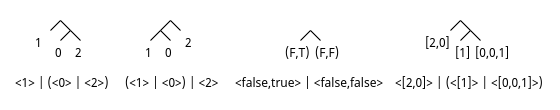
\includegraphics[width=0.9\textwidth]{../images/tree-example.png}
	\caption{Building binary trees of naturals, pairs and lists}
	\label{fig:tree-example}
\end{figure}

Iteration on trees is similar to iteration on lists. The first argument of \verb$iteTree$ is a function that can turn a leaf of type \verb$A$ to some term \verb$B$. The second argument is a function that, given the two partial results from the recursive processing of the left and right subtrees, gives us a new result. Finally, the third argument is the tree itself to iterate. Code \ref{code:examples-tree-eval} shows some example computations on trees.

\begin{listing}[H]
\begin{minted}{agda}
size = "(λ t. iteTree ((λ_. 1):ℕ→ℕ) (λ l r. l + r) t) : (Tree ℕ) → ℕ"

_ : eval (size ++ₛ "<3>")                        ≡ inj₁ (Nat , λ γ* → 1)
_ : eval (size ++ₛ "<3> | ((<10> | <2>) | <3>)") ≡ inj₁ (Nat , λ γ* → 4)

sum = "(λ t. iteTree ((λx. x):ℕ→ℕ) (λ l r. l + r) t) : (Tree ℕ) → ℕ"

_ : eval (sum  ++ₛ "<3>")                        ≡ inj₁ (Nat , λ γ* → 3)
_ : eval (sum  ++ₛ "<3> | ((<10> | <2>) | <3>)") ≡ inj₁ (Nat , λ γ* → 18)

map = "(λ f t. iteTree ((λx.<f x>):ℕ→(Tree 𝕃)) (λ l r. l | r) t)
      : (ℕ → 𝕃) → (Tree ℕ) → (Tree 𝕃)"

_ : eval (map ++ₛ even ++ₛ "(<0> | <7>) | (<1> | <10>)") ≡
    inj₁ (Ty.Tree Bool ,
    λ γ* → Tree.node (Tree.node (Tree.leaf tt) (Tree.leaf ff))
                     (Tree.node (Tree.leaf ff) (Tree.leaf tt)))
\end{minted}
\caption{Example: tree operations and their evaluation}
\label{code:examples-tree-eval}
\end{listing}

Coinductive types are the mathematical dual of inductive types. They are specified by their destructors, also often called \textit{observers}, which most of the time, either return a simpler type, or a new copy of the original object with a different inner state. Our STLC implementation features two coinductive type formers: \verb$Stream$ and \verb$Machine$.

\begin{listing}[H]
\begin{minted}{agda}
evens = "genStream ((λn.n):ℕ→ℕ) (λn.n+2) 0"
odds  = "genStream ((λn.n):ℕ→ℕ) (λn.n+2) 1"

_ : eval ("head"           ++ evens) ≡ inj₁ (Nat , λ γ* → 0)
_ : eval ("head tail"      ++ evens) ≡ inj₁ (Nat , λ γ* → 2)
_ : eval ("head tail tail" ++ evens) ≡ inj₁ (Nat , λ γ* → 4)
_ : eval ("head"           ++ odds)  ≡ inj₁ (Nat , λ γ* → 1)
_ : eval ("head tail"      ++ odds)  ≡ inj₁ (Nat , λ γ* → 3)
_ : eval ("head tail tail" ++ odds)  ≡ inj₁ (Nat , λ γ* → 5)
\end{minted}
\caption{Example: infinite streams of even and odd numbers}
\label{code:examples-streams-1}
\end{listing}

\verb$genStream$ introduces stream types from three arguments. A \textit{seed}, or \textit{initial state}, which is the third argument. A function, which specifies how the \verb$head$ eliminator must turn a stream state to a result. Finally, a specification for the \verb$tail$ operation that "advances the stream", i.e., produces a new state from the previous. In the case of \verb$even$ and \verb$odd$, the seeds and the operations are all trivial as seen on Code \ref{code:examples-streams-1}.

\begin{listing}[H]
\begin{minted}{agda}
first-n = "genStream ((λns.ns):[ℕ]→[ℕ]) (λ ns. (" ++ length ++ " ns) ∷ ns)
                                                               (nil : [ℕ])"

_ : eval ("head"          ++ first-n) ≡ inj₁ (Ty.List Nat , (λ γ* → []))
_ : eval ("head tail"     ++ first-n) ≡ inj₁ (Ty.List Nat , (λ γ* → 0 ∷ []))
_ : eval ("head tail tail" ++ first-n) ≡ inj₁ (Ty.List Nat , (λ γ* → 1 ∷ (0 ∷ [])))

step-n = "(λ start diff. genStream ((λn.n):ℕ→ℕ) (λn. n+diff) start)
                                                     : ℕ → ℕ → (Stream ℕ)"

_ : eval ("head           ((" ++ step-n ++ ") 10) 5") ≡ inj₁ (Nat , λ γ* → 10)
_ : eval ("head tail      ((" ++ step-n ++ ") 10) 5") ≡ inj₁ (Nat , λ γ* → 15)
_ : eval ("head tail tail ((" ++ step-n ++ ") 10) 5") ≡ inj₁ (Nat , λ γ* → 20)

_ : eval ("head           ((" ++ step-n ++ ") 0) 33") ≡ inj₁ (Nat , λ γ* → 0)
_ : eval ("head tail      ((" ++ step-n ++ ") 0) 33") ≡ inj₁ (Nat , λ γ* → 33)
_ : eval ("head tail tail ((" ++ step-n ++ ") 0) 33") ≡ inj₁ (Nat , λ γ* → 66)

get-nth = "(λ s n. head iteℕ s (λ ss. tail ss) n) : (Stream ℕ) → ℕ → ℕ"

_ : eval (get-nth ++ₛ odds  ++ₛ  "8") ≡ inj₁ (Nat , λ γ* → 17)
_ : eval (get-nth ++ₛ evens ++ₛ "13") ≡ inj₁ (Nat , λ γ* → 26)

_ : eval ("((" ++ get-nth ++ ") (((" ++ step-n ++ ") 100) 25))" ++ "3") ≡
                                                inj₁ (Nat , λ γ* → 175)
_ : eval ("((" ++ get-nth ++ ") (((" ++ step-n ++ ")   0) 30))" ++ "5") ≡
                                                inj₁ (Nat , λ γ* → 150)
\end{minted}
\caption{Example: arithmetic progression and parametric streams}
\label{code:examples-streams-2}
\end{listing}

\verb$first-n$ generates the (decreasing) sequences of first \verb$n$ natural numbers \verb$(n ∈ ℕ)$: \verb$[]$, \verb$[0]$, \verb$[1,0]$, \verb$[2,1,0]$, etc.

\verb$step-n$ is a function that takes two naturals, \verb$start$ and \verb$diff$, and returns a stream that generates the arithmetic progression, which starts at \verb$start$ and where the difference is \verb$diff$.

Finally, \verb$get-nth$ is a function that takes a stream of naturals and an index \verb$n$, and returns the nth element from the stream, i.e., it applies \verb$n$ number of \verb$tail$ destructors, then a \verb$head$. For this, we use \verb$iteℕ$: we iterate on the parameter \verb$n$; replace \verb$zero$ with the stream parameter; and replace each \verb$suc$ with a \verb$tail$. For example, with \verb$n=3$ the following informal rewriting happens:\\
\verb$get-nth s suc(suc(suc(zero))) ⟶  head tail tail tail s$

Our \verb$Machine$ type works like simple state machines with the following semantics:

\begin{itemize}
	\item{\verb$put$: taking the current state and a number, it advances the state - \textit{input}}
	\item{\verb$set$: advances the state - \textit{signal}}
	\item{\verb$get$: produces a natural number from the current state and returns it - \textit{output}}
	\item{\verb$seed$: initial state, which has an arbitrary type, like with \verb$Stream$}
\end{itemize}

\begin{listing}[H]
\begin{minted}{agda}
sum-machine = "genMachine (λs i. s+i) (λ_.0) (λs.s) 0"

_ : eval ("get "                 ++ sum-machine)          ≡ inj₁ (Nat , λ γ* →  0)
_ : eval ("get put "             ++ sum-machine ++ " 10") ≡ inj₁ (Nat , λ γ* → 10)
_ : eval ("get put put put "     ++ sum-machine ++ " 10 20 30")
                                                          ≡ inj₁ (Nat , λ γ* → 60)
_ : eval ("get put put set put " ++ sum-machine ++ " 10 20 30")
                                                          ≡ inj₁ (Nat , λ γ* → 50)
\end{minted}
\caption{Example: Machine for summation}
\label{code:examples-machines-1}
\end{listing}

Code \ref{code:examples-machines-1} presents a simple example. \verb$sum-machine$, starting from zero, adds together all numbers input with \verb$put$. \verb$get$ can be used to extract the result, and \verb$set$ to reset the sum to zero.

\begin{listing}[H]
\begin{minted}{agda}
partitioned-sums = "genMachine                                                  \
\                     (λs i. if (" ++ even ++ "i) then                          \
\                       ((fst s) ,  (fst snd s)      , ((snd snd s) + i))       \
\                     else                                                      \
\                       ((fst s) , ((fst snd s) + i) ,  (snd snd s)    ))       \
\                     (λs. (" ++ not ++ "(fst s)) , (fst snd s) , (snd snd s))  \
\                     (λs. if (fst s) then (fst snd s) else (snd snd s))        \
\                     (true , 0 , 0)"

_ : eval ("get put put put put"     ++ partitioned-sums ++ "3 10 1 8") ≡
                                                          inj₁ (Nat , λ γ* → 4)
_ : eval ("get put put put put set" ++ partitioned-sums ++ "3 10 1 8") ≡
                                                          inj₁ (Nat , λ γ* → 18)
\end{minted}
\caption{Example: Machine that sums odd and even numbers separately}
\label{code:examples-machines-2}
\end{listing}

\verb$partitioned-sums$ works like \verb$sum-machine$, except it adds together the even and odd numbers separately. Also, now the purpose of \verb$set$ is to toggle a boolean flag, that determines which sum \verb$get$ will return. To implement this, we used products to store a triple as internal state: \textit{(flag, odd-sum, even-sum)}. In \verb$put$, we add to the 2nd or 3rd component of the state depending on the \verb$even$ check's result. \verb$set$ toggles the first component and does not touch the other two. \verb$get$ returns the 2nd or 3rd depending on the flag component's state.

At this point, the reader can see that constructing inner states of arbitrary complexity is possible. Also, we could support "machine types" which have more than one input methods (like \verb$put$), output methods (like \verb$get$) and signals (like \verb$set$); essentially simulating constructions like Turing machines, REPLs or even operating systems.


\cleardoublepage

\chapter{Conclusion}
\label{ch:conclusion}

\section{Results}

This thesis has introduced readers to the formalisation of a small language based on simply typed \verb$λ$-calculus. We guided them through each elaboration step of the language, going from source code to well-typed terms and interpretation results. The steps include lexing, parsing, scope checking, type checking and a meta theoretic interpretation that serves as a form of semantical evaluation. We presented algebraic definitions and total conversions between them, formalised in Agda for a solution that is correct by construction. We picked conventional and well-known syntactic elements for both the base STLC constructions and its included extensions.

This study also explains some inductive types like lists and trees, formal definitions for their iteration, as well as implementations of some standard functions on them. We also briefly touched upon coinductive types, along their introduction and elimination rules through our \verb$Stream$ and \verb$Machine$ types.

Our framework provides an easy to use interface consisting of a small set of high-level functions for users to test and experiment on STLC terms. We report errors encountered on various levels of the elaboration stack, e.g., syntax errors, scope errors and type errors.

Our codebase remains publicly accessible for anyone on GitHub and is open for future study and development \cite{home-repo}.

\section{Discussion}

At an early stage of development, we limited our type annotations to lambda terms, which we called "annotated lambdas". This meant that each variable binding in a lambda could be annotated, so we wrote \verb$"λx:ℕ y:ℕ.x+y"$ instead of \verb$"(λx y.x+y):ℕ→ℕ"$. This worked, however, we later realised that lambdas are not the only terms that need type annotations. For example, the empty list, \verb$nil$, or terms of sum types like \verb$inl true$, also need annotation, otherwise it is impossible to infer their complete types. That is why we dropped our "annotated lambda" syntax and introduced the general type annotation for arbitrary terms instead.

Note that the "annotated lambda" method is similar to Church's STLC definition, where abstractions have \textit{domains}, e.g., \verb$λx:σ.M$; opposed to Curry's one, which would instead write \verb$λx.M : σ→σ$ \cite{sorensen1998curry}.

Performance is definitely not the strong suit of our elaborator. Type checking of files with a few dozen examples, or ones with slightly more complex constructions, such as \verb$partitioned-sums$, sometimes took up to a minute on average hardware. We suspect that this is due to the high amount of implicit arguments Agda has to lookup and substitute. It is not obvious which part of the elaboration stack would be a good target for optimisation. Benchmarking shows that parsing takes a substantial amount of time, so it might be a good candidate. Type checking could potentially be smarter if we included some "optimisation steps", ones like simplification using the \verb$η$-reduction principle, turning \verb$lam q [ p ] $\verb$$\verb=$=\verb$$\verb$ q$ to \verb$lam q$. This way Agda would get structurally smaller terms earlier.

\section{Future work}

We already touched on the idea of injecting a lexer independent of agdarsec into our toolchain. The main demand for this comes from the fact that the one parametrised with the functions \verb$keyword$, \verb$breaking$ and \verb$default$ cannot fail. This currently results in overly permissive variable names and an unused \verb$lexical-error$ case in the elaboration.

There are many aspects we could improve upon our parser. A cleverer implementation would probably spare us some parentheses. For example, function application always requires one, like in \verb$"((λx.x):ℕ→ℕ) 1"$. This so far, looks reasonable, but looks less right once we apply more than one arguments: \verb$"(((λx y.x+y):ℕ→ℕ→ℕ) 1) 2"$. Solving this in the total parser however, is not a trivial task.

Less obvious is the fact that type inference could also be improved upon. Here we mean that a smarter implementation would alleviate the need for many type annotations. For example, as discussed previously, it is reasonable to expect annotation for \verb$"λx.x"$, since \verb$x$ can be any type and we do not support polymorphic functions. However, if we look at \verb$"λx.isZero x"$, it is apparent that \verb$x$ must be \verb$ℕ$ for the term to be type correct. Dual to this is the case where we would have to analyse not the body, but the context of the abstraction, like in \verb$"(λx.x) 3"$. Here it is obvious that the function's type must be \verb$ℕ→ℕ$. The current implementation, as shown on Code \ref{code:typecheck-infer-lam}, first infers the type of the function and then checks whether the argument has the correct type, not the other way around. It might be reasonable to implement a solution that tries both ways of inference and checking to lower the number of function type annotations required.

The framework would entail a considerably more complete study, if we also included a normalisation of our own. We briefly mentioned this in Chapter \ref{sec:normalisation}. It could be a future update merge from the formalisation codebase we initially forked from \cite{typesystems-repo}, if the normalisation ever got finished.

An even greater undertaking would be to boost the expressibility of the presented language by introducing higher order concepts, like type polymorphism or full recursion for the function space by using some form of fixpoint combinator.


\cleardoublepage

% Acknowledgements (optional) - in case your thesis received funding or would like to express special thanks to someone
\chapter*{\acklabel}
\addcontentsline{toc}{chapter}{\acklabel}
TODO

% Appendices (optional) - useful for detailed information in long tables, many and/or large figures, etc.
%\appendix
%\input{chapters/app.tex}
%\cleardoublepage

% Bibliography (mandatory)
\phantomsection
\addcontentsline{toc}{chapter}{\biblabel}
\printbibliography[title=\biblabel]
\cleardoublepage

% List of figures (optional) - useful over 3-5 figures
\phantomsection
\addcontentsline{toc}{chapter}{\lstfigurelabel}
\listoffigures
\cleardoublepage

% List of tables (optional) - useful over 3-5 tables
\phantomsection
\addcontentsline{toc}{chapter}{\lsttablelabel}
\listoftables
\cleardoublepage

% List of algorithms (optional) - useful over 3-5 algorithms
\phantomsection
\addcontentsline{toc}{chapter}{\lstalgorithmlabel}
\listofalgorithms
\cleardoublepage

% List of codes (optional) - useful over 3-5 code samples
\phantomsection
\addcontentsline{toc}{chapter}{\lstcodelabel}
\lstlistoflistings
\cleardoublepage

% List of symbols (optional)
% Add notation like this later:
%\nomenclature{\(Γ\)}{Arbitrary context}
%\nomenclature{\(◇\)}{Empty context}
\printnomenclature

\end{document}
